\section*{Analiza porównacza wyjaśnień}
W tej sekcji przeprowadzono analizę porównawcą wyjaśnień generowanych przez różne metody XAI: LIME, SHAP i GradCAM.

Analiza została przeprowadzona na trzech poziomach:
\begin{enumerate}
	\item \textbf{Na całym zbiorze danych}, w celu zrozumienia ogólnej skuteczności każdej z metod XAI.
	\item \textbf{Z podziałem na kategorie obrazów}, w celu zbadania, jak różne typy obiektów wpływają na spójność wyjaśnień.
	\item \textbf{W zależności od wielkości obiektów na obrazie}, aby zbadać, czy rozmiar obiektu ma wpływ na spójność wyjaśnień oraz jakie obszary obrazu są istotne dla różnych metod XAI.
\end{enumerate}

Celem tej analizy było zrozumienie, które metody XAI są najbardziej skuteczne w identyfikacji istotnych cech orazów oraz jakie czynniki mogą wpłynąć na spójność i stabilność wyjaśnień generowanych przez metody.
Każda z tych metod ma inne teoretyczne podstawy oraz praktyczne założenia, które mogą istotnie wpływać na ich skuteczność i użyteczność w różnych zastosowaniach.
Dzięki temu możliwe jest lepsze zrozumienie mechanizmów działania każdej z metod i ich potencjalnych zastosowań w praktyce.

\subsection*{Analiza na całym zbiorze danych}.

W tej części przeprowadzono analizę porównawczą metod XAI na całym zbiorze danych, w celu zbadania ogólnych właściwości oraz efektywności metod XAI w kontekście wyjaśniania modeli głębokich.
Skupiono się na ocenie Intersection over Union, procentowego udziału obszaru wyjaśnienia poza obiektem oraz zmianach w pewności modelu po zastosowaniu wyjaśnień.

\vspace{1cm}

Analiza porównawcza wartości IoU dla wybranych metod na całym zbiorze danych dostarczyła inforamcji na dotyczących spójności generowanych wyjaśnień z danymi prawdziwymi.

\begin{figure}[h]
	\centering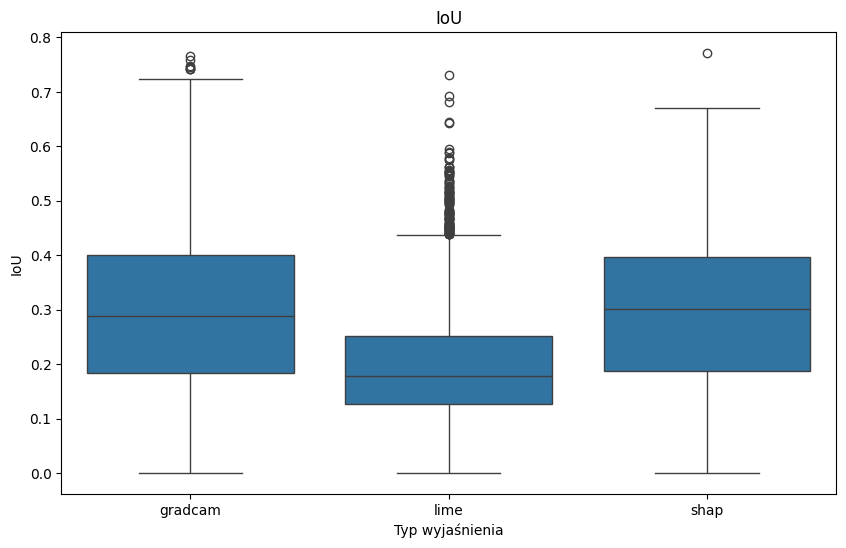
\includegraphics[width=.9\textwidth]{img/base_iou}
	\caption{Wartości IoU  dla stosowanych obrazów}  \label{rys:basiciou}
\end{figure}

\begin{table}[h]
	\centering
	\begin{tabular}{|c|c|c|c|}
		\hline
		\textbf{Metoda XAI}  & \textbf{GradCAM} & \textbf{LIME} & \textbf{SHAP} \\
		\hline
		\textbf{Średnie IoU} & 0.439863         & 0.176337      & 0.118810      \\
		\hline
	\end{tabular}
	\caption{Średnie wartości IoU}
	\label{tab:basiciou}
\end{table}


Wyniki analizy pokazano na wykresie pudełkowym (Rys. \ref{rys:basiciou}), który przedstawia rozkład wartości IoU dla poszczególnych metod XAI.
Dodatkowo, Tabela \ref{tab:basiciou} zawiera średnie wartości IoU dla każdej z metod.

Najwyższym wynikiem IoU wykazał się \textbf{GradCAM}, co wskazuje na wysoką zgodnośc wyjaśnień z rzeczywistymi obszarami decyzyjnymi modelu.

\textbf{LIME} uzyskał IoU na niższym poziomie, co sugeruje, że wyjaśnienia generowane przez LIME często pokrywają mniejsze obszary obiektów na obrazach.
Może to być spowodowanem doborem jednakowych parametrów niezależnie od obrazu.

\textbf{SHAP} wykazał najniższe wartości IoU w porównaniu do innych metod.

Analiza IoU pokazała, że GradCAM oferuje największą spójnośc i zgodność wyjaśnień z rzeczywistymi obszarami decyzyjnymi modelu.
LIME i SHAP osiągnęły gorsze wyniki co może być spowodowane doborem parametrów oraz metodą dostarczania wyjaśnień, wyjaśnienia są mniejsze oraz często skupiają się na koknkretnych cechach obiektu, nie na całym obiekcie.

\vspace{1cm}

W celu dostarczenia dodatkowych informacji o spójności wyjaśnień, zbadano jaki procent obszaru wyjaśnienia znajduje się poza obiektem, czyli jest nieprawidłowo oznaczony.
Analiza ta ma nacelu ocenę precyzji lokalizacji wyjaśnień generowanych przez LIME, SHAP i GradCAM na całym zbiorze danych ImageNet-9.

\begin{figure}[h]
	\centering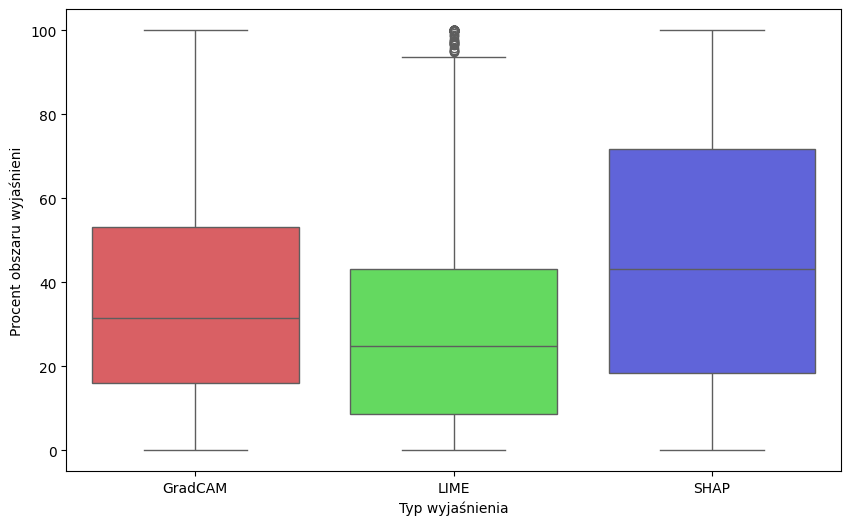
\includegraphics[width=.9\textwidth]{img/areaincorrect}
	\caption{Procent obszaru wyjaśnienia poza obiektem}  \label{rys:areaincorrect}
\end{figure}

\begin{table}[h]
	\centering
	\begin{tabular}{|c|c|c|c|}
		\hline
		\textbf{Metoda XAI}                          & \textbf{GradCAM} & \textbf{LIME} & \textbf{SHAP} \\
		\hline
		\textbf{Średni procent obszaru wyjaśnienia } & 36.310489\%      & 28.544654\%   & 45.590079\%   \\
		\hline
	\end{tabular}
	\caption{Procent obszaru wyjaśnienia poza obiektem}
	\label{tab:areaincorrect}
\end{table}

Wyniki analizy pokazano na wykresie pudełkowym (Rys. \ref{rys:areaincorrect}), który przedstawia rozkład wartości procentów obszarów wyjaśnienia poza obiektem poszczególnych metod XAI.
Dodatkowo, Tabela \ref{tab:areaincorrect} zawiera średnie procenty obszarów wyjaśnień poza obiektem.

Analiza wykazała, że najlepszy wynik osiągnął \textbf{LIME}.
Oznacza to, że metoda ta generuje wyjaśnienia o najmniejszym rozproszeniu, koncentrując się na istotnych cechach obiektów.

\textbf{GradCAM} pomimo wysokiego IoU, osiągnął gorsze wyniki pod względem procentu obszru wyjaśnieńia poza obiektem.
Może być to spowodowane wyjaśnieniami generowanymi na superpiksele, związane z wielkością ostatniej warstwy konwolucyjnej, co może prowadzić do uwzględnienia obszarów obrazu, które są bezpośrednio związane z rzeczywistyi obiektami.

Najgorsze wyniki w tej analizie osiągnął \textbf{SHAP}, co może być związne z wrażliwością tej metody na hiperparametry.

Analiza procentu obszaru wyjaśnienia poza obiektem pokazuje, że LIME generuje wyjaśnienia o najmniejszym rozproszeniu, skupiając się na istotnych cech.
GradCAM przez sposób dostarczania wyjaśńień, wyjaśnienia często posiadają obszary spoza rzeczywistego obiektu.
SHAP przez wrażliwość na hiperparametry posiadał najgorsze wyniki.

\vspace{1cm}

W tej częsci przeprowadzono analiza porównawcza zmiany pewności modelu po pozostawieniu jedynie obszaru wyjaśnień generowanych przez wybrane metody XAI. 
Celem analizy było zrozumienie, w jaki sposób wyjaśnienia wpływają na pewność decyzji modelu głębokiego uczenia.

\begin{figure}[h]
	\centering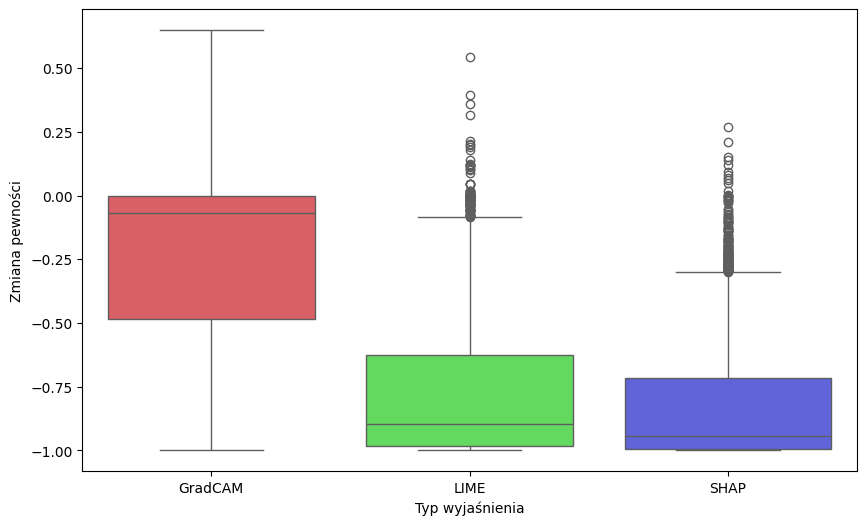
\includegraphics[width=.9\textwidth]{img/base_confidence_exp}
	\caption{Zmiana pewności po pozostawieniu jedynie obszaru wyjaśnienia}  \label{rys:base_confidence_exp}
\end{figure}

\begin{table}[h]
	\centering
	\begin{tabular}{|c|c|c|c|}
		\hline
		\textbf{Metoda XAI}             & \textbf{GradCAM} & \textbf{LIME} & \textbf{SHAP} \\
		\hline
		\textbf{Średni spadek pewności} & -0.247974        & -0.781209     & -0.826915     \\
		\hline
	\end{tabular}
	\caption{Średni spadek pewności modelu po pozostawieniu jedynie obszaru wyjaśnienia}
	\label{tab:base_confidence_exp}
\end{table}

\begin{table}[h]
	\centering
	\begin{tabular}{|c|c|c|c|}
		\hline
		\textbf{Metoda XAI} & \textbf{GradCAM} & \textbf{LIME} & \textbf{SHAP} \\
		\hline
		\textbf{Procent}    & 24.8148\%        & 0.8642\%      & 0.2963\%      \\
		\hline
	\end{tabular}
	\caption{Procent przytaków, w których pewność się zwiększyła}
	\label{tab:base_confidence_exp_percent}
\end{table}

Wyniki analizy przedstawiono na wykresie (Rys. \ref{rys:base_confidence_exp}), który ilustruje zmianę pewności modelu po pozostawieniu jedynie obszarów wyjaśnień.
Dodatkowo Tabela \ref{tab:base_confidence_exp} przedstawia średni spadek pewności modelu dla każdej z metod, natomiast Tabela \ref{tab:base_confidence_exp_percent} pokazuje procent przypadków, w których pewność modelu wzrosła po zastosowaniu wyjaśnień.

\textbf{GradCAM} wykazał najmniejszy spadek pewnośći oraz największy procent przypadków, w których pewność wzrosła.
Jest to zgodne z oczekiwaniami ponieważ wyjaśnienia GradCAM są często większe i skupiają się na całym obiekcie.
Natomiast\textbf{SHAP} i\textbf{LIME} uzyskały niższe wyniki w tej analizie, co może wynikać z tendencji wybierania mniejszych obszarów wyjaśnień, co prowadzi do mniejszego wpływu na pewność modelu.  

\vspace{1cm}

Analiza porównawcza zmiany pewności decyzji po usunięciu wyjaśnionych obszarów dla metod GradCAM, LIME i SHAP dostarczyła informacji dotyczące wpływu interpretacji na pewność modelu.

\begin{figure}[h]
	\centering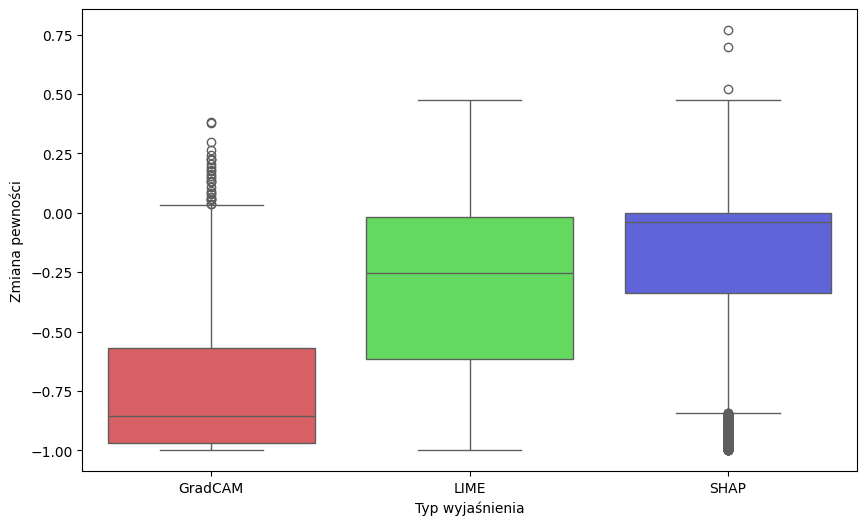
\includegraphics[width=.9\textwidth]{img/base_confidence_no_exp}
	\caption{Zmiana pewności po usunięciu obszaru wyjaśnienia}  \label{rys:base_confidence_no_exp}
\end{figure}

\begin{table}[h]
	\centering
	\begin{tabular}{|c|c|c|c|}
		\hline
		\textbf{Metoda XAI}              & \textbf{GradCAM} & \textbf{LIME} & \textbf{SHAP} \\
		\hline
		\textbf{Średnia zmiana pewności} & -0.747604        & -0.342071     & -0.204317     \\
		\hline
	\end{tabular}
	\caption{Średni spadek pewności modelu po usunięciu obszaru wyjaśnienia}
	\label{tab:base_confidence_no_exp}
\end{table}

Wyniki analizy przedstawiono na wykresie (Rys. \ref{rys:base_confidence_no_exp}), który ilustruje zmianę pewności modelu po usunięciu obszaru wyjaśnienia.
Natomiast Tabela \ref{tab:base_confidence_no_exp} przedstawia średni spadek pewności modelu dla każdej z metod.

Najlepsze wyniki uzyskał \textbf{GradCAM}, co wskazuje na duży wpływ obszaru wyjaśnienia na decyzję modelu.

\textbf{LIME} wygenerował mniejsze zmiany w pewności, co może wynikać z tendencji do generowania mniejszych wyjaśnień.

Z kolei \textbf{SHAP} wygenerował najmniejszy spadek, co może być spowodowane generowaniem mniejszych wyjaśnień oraz wysokiej czułości na hiperparametry.

Analiza zmiany pewności decyzji po usunięciu obszarów wyjaśnień wykazała, że metoda GradCAM generuje wyjaśnienia z obszarami wysoce wpływającymi na pewność modelu.
Natomiast zarówno LIME jak i SHAP generują wyjaśnienia z obszarami sumarycznie mniej ważnymi.

\subsection*{Analiza z podziałem na kategorie obrazu}

W tej części przeprowadzono analizę porównawczą metod XAI z podziałem na wybrane kategorie obrazów.
Celem badania było dokładniejsze zrozumienie różnic w jakości wyjaśnień oraz ocena wpływu kategorii obrazu na wyniki.
Każda technika XAI może reagować inaczej na różne typy obiektów, co może mieć istotne znaczenie dla ich zastosowań w praktyce.

\begin{figure}[h]
	\centering
	\begin{subfigure}[b]{0.3\textwidth}
		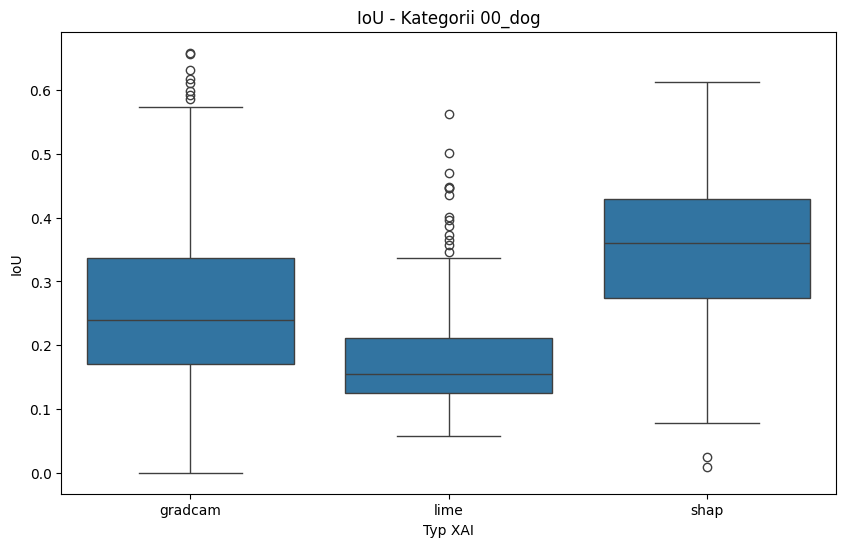
\includegraphics[width=.9\textwidth]{img/base_iou_dog}
		\caption{Dog}
	\end{subfigure}
	\begin{subfigure}[b]{0.3\textwidth}
		\centering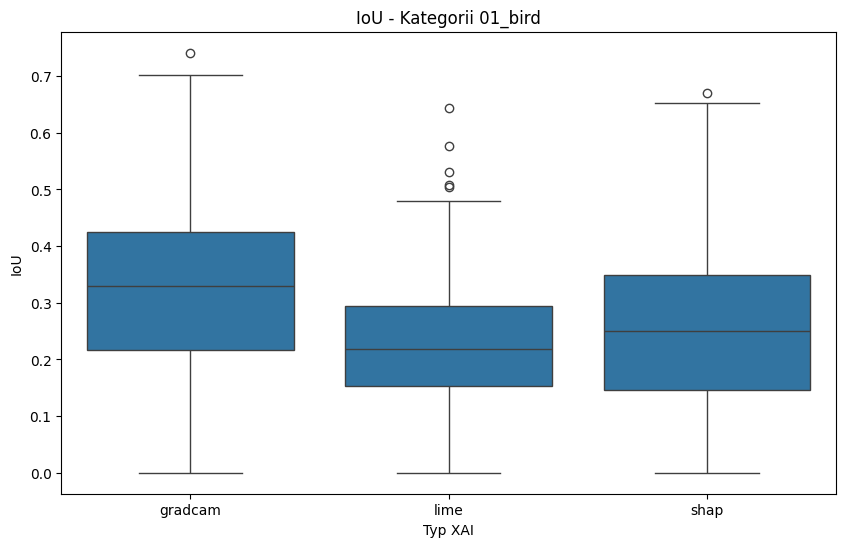
\includegraphics[width=.9\textwidth]{img/base_iou_bird}
		\caption{Bird}
	\end{subfigure}
	\begin{subfigure}[b]{0.3\textwidth}
		\centering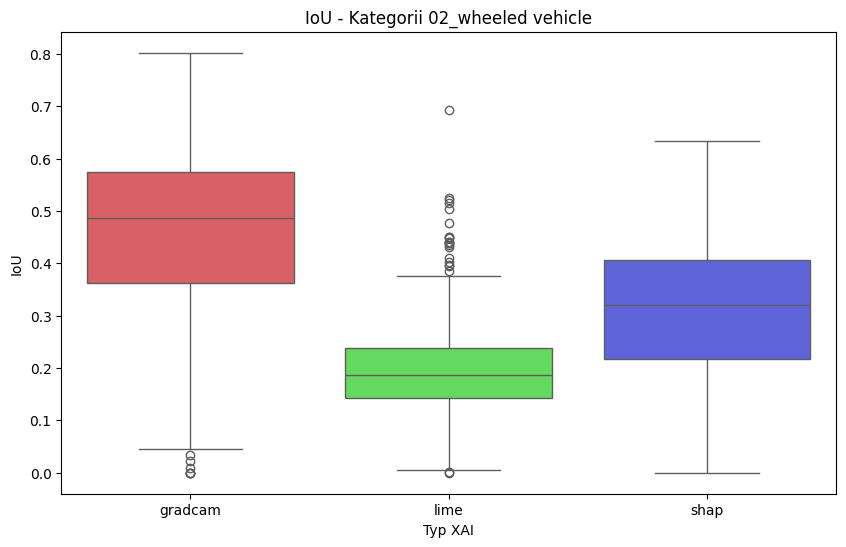
\includegraphics[width=.9\textwidth]{img/base_iou_vehicle}
		\caption{Vehicle}
	\end{subfigure}
	\begin{subfigure}[b]{0.3\textwidth}
		\centering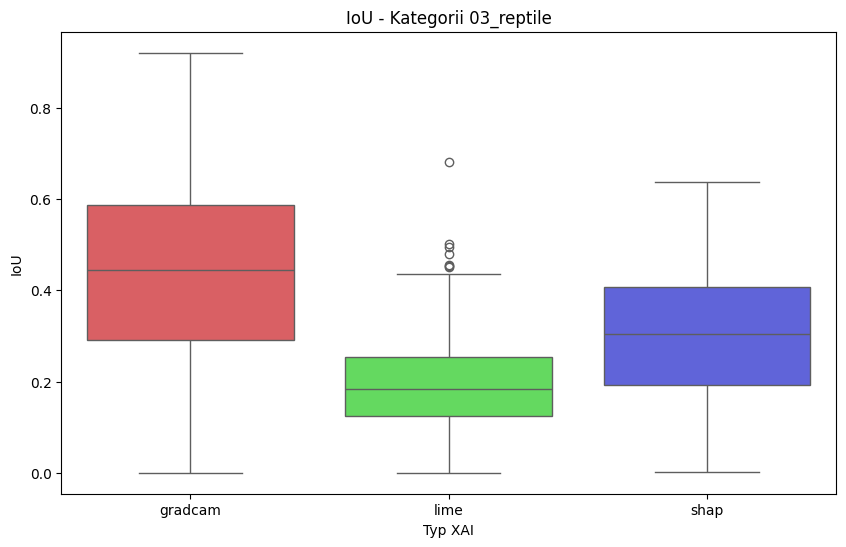
\includegraphics[width=.9\textwidth]{img/base_iou_reptile}
		\caption{Reptile}
	\end{subfigure}
	\begin{subfigure}[b]{0.3\textwidth}
		\centering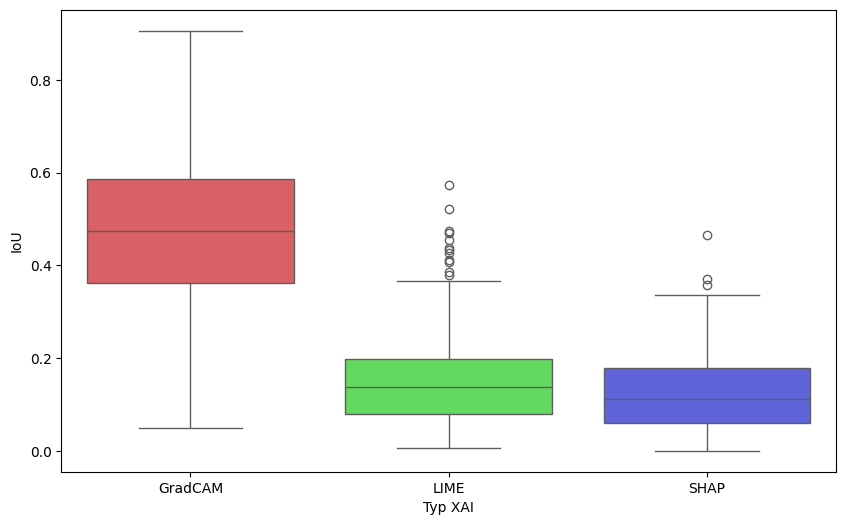
\includegraphics[width=.9\textwidth]{img/base_iou_carnivore}
		\caption{Carnivore}
	\end{subfigure}
	\begin{subfigure}[b]{0.3\textwidth}
		\centering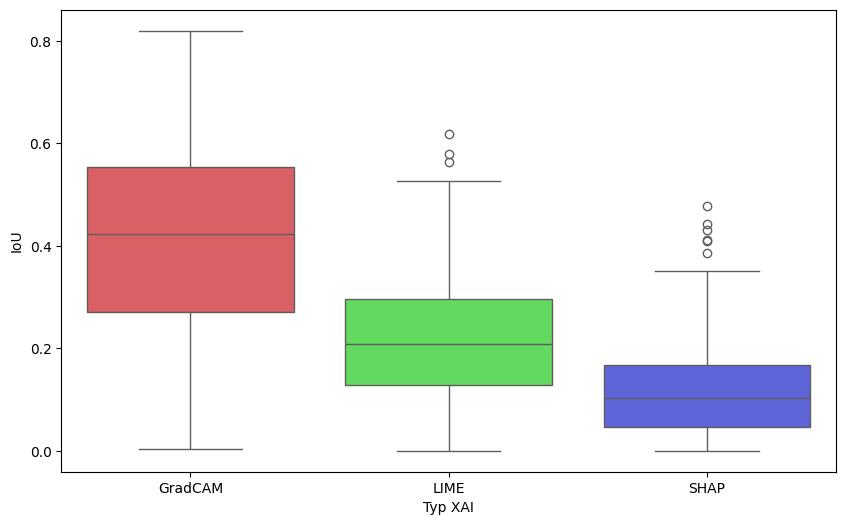
\includegraphics[width=.9\textwidth]{img/base_iou_insect}
		\caption{Insect}
	\end{subfigure}
	\begin{subfigure}[b]{0.3\textwidth}
		\centering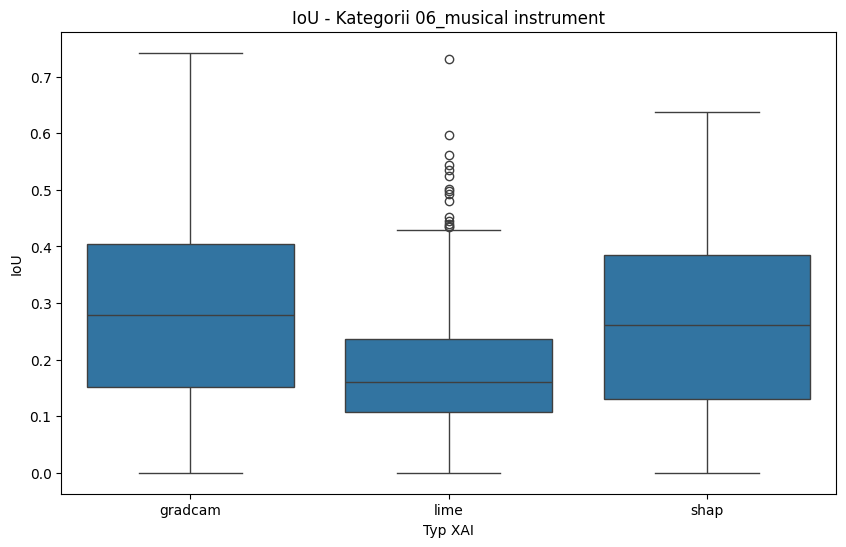
\includegraphics[width=.9\textwidth]{img/base_iou_music}
		\caption{Instrument}
	\end{subfigure}
	\begin{subfigure}[b]{0.3\textwidth}
		\centering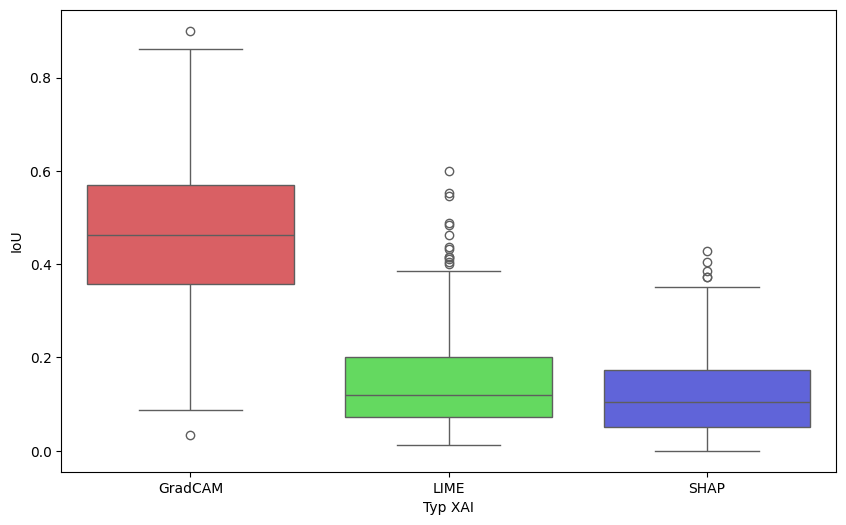
\includegraphics[width=.9\textwidth]{img/base_iou_primate}
		\caption{Primate}
	\end{subfigure}
	\begin{subfigure}[b]{0.3\textwidth}
		\centering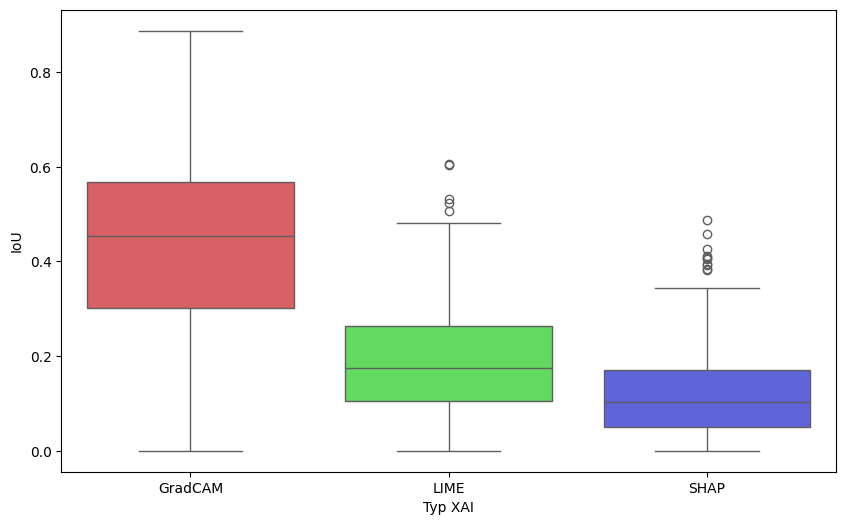
\includegraphics[width=.9\textwidth]{img/base_iou_fish}
		\caption{Fish}
	\end{subfigure}
	\caption{Wartości IoU dla różnych kategorii obrazów}
	\label{rys:base_iou_category}
\end{figure}

\begin{table}[h]
	\centering
	\begin{tabular}{|c|c|c|c|}
		\hline
		\textbf{Kategoria}           & \textbf{GradCAM} & \textbf{LIME} & \textbf{SHAP} \\
		\hline
		\textbf{Pies}                & 0.467134         & 0.140748      & 0.123451      \\
		\hline
		\textbf{Ptak}                & 0.428416         & 0.166958      & 0.123881      \\
		\hline
		\textbf{Pojazd na kołach}    & 0.459880         & 0.185348      & 0.121152      \\
		\hline
		\textbf{Gad}                 & 0.436193         & 0.201811      & 0.121951      \\
		\hline
		\textbf{Mięsożerca}          & 0.468916         & 0.154079      & 0.122430      \\
		\hline
		\textbf{Insekt}              & 0.410650         & 0.218640      & 0.115746      \\
		\hline
		\textbf{Instrument muzyczny} & 0.394289         & 0.179295      & 0.102792      \\
		\hline
		\textbf{Naczelny}            & 0.465292         & 0.150706      & 0.118099      \\
		\hline
		\textbf{Ryba}                & 0.427992         & 0.189446      & 0.113783      \\
		\hline
	\end{tabular}
	\caption{IoU dla kategorii}
	\label{tab:base_iou_category}
\end{table}

Wyniki analizy IoU w zależności od kategorii obrazów przedstawiono na wykresach (Rys. \ref{rys:base_iou_category}) oraz w Tabeli \ref{tab:base_iou_category}, która zawiera średnie wartości IoU dla poszczególnych metod XAI i kategorii.

Metoda \textbf{GradCAM} osiąga najlepsze wyniki niezależnie od wybranej kategorii obrazu, co świadczy o jej zdolności do lokalizowania rzeczywistego obiektu.
Najwyższe wartości osiągnęła dla kategorii \textit{Mięsożerca} oraz \textit{Pies}.
Najniższe natomiast dla kategorii \textit{Instrument muzyczny}.

Metoda \textbf{LIME} uzyskuje niższe wartości IoU w porównaniu do GradCAM.
Najwyższe wyniki LIME zaobserwowano dla kategorii \textit{Insekt}.
Najniższe natomiast dla kategorii \textit{Pies}.

Metoda \textbf{SHAP} uzyskuje podobne wartości niezależnie od wybranej kategorii.
Przy czym najlepsze wyniki dla kategorii \textit{Ptak}.
Natomiast najgorsze dla kategorii \textit{Instrument muzyczny}.

Jedyną kategorią dla której średnia wartość IoU jest większa dla wszystkich wyjaśniń od średniej wartości dla całego zbioru jest kategoria \textit{Pojazd na kołach}.
Natomiat żadna kategoria nie jest gorsze dla wszystkich wyjaśnień.

Metoda GradCAM wykazuje się najwyższą spójnością i precyzją w generowaniu wyjaśnień.
Zarówno LIME jak i SHAP generują wyjaśnienia o niższej spójności.

\vspace{1cm}

Anlize średniego procentu obszaru wyjaśnienia poza obiektem pozwoliła nalepsze zrozumienie wyników IoU.

\begin{figure}[h]
	\centering
	\begin{subfigure}[b]{0.3\textwidth}
		\centering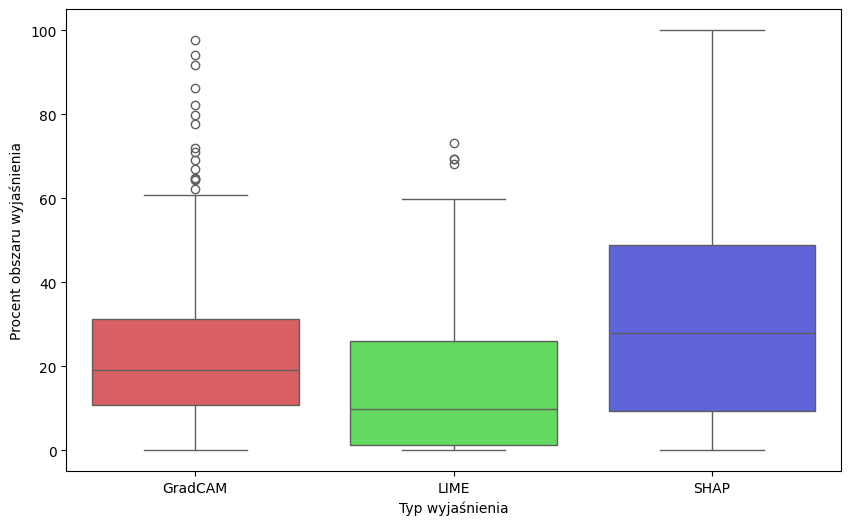
\includegraphics[width=.9\textwidth]{img/areaincorrect_dog}
		\caption{Dog}
	\end{subfigure}
	\begin{subfigure}[b]{0.3\textwidth}
		\centering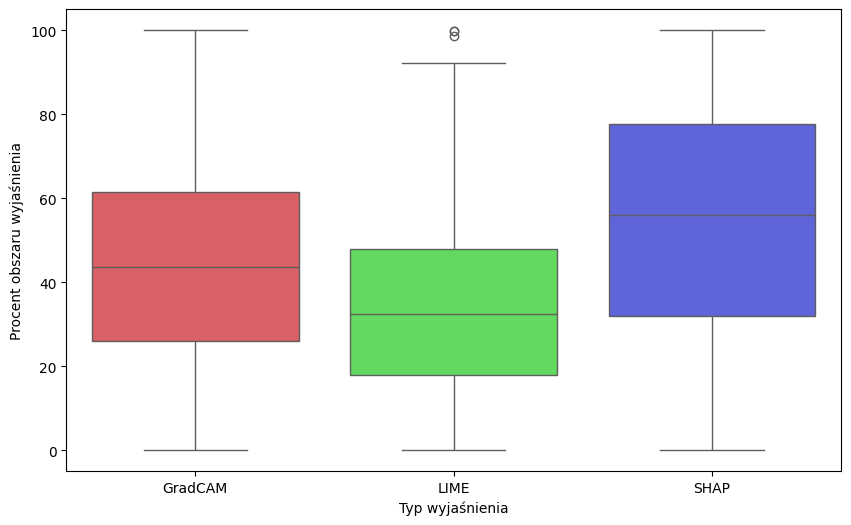
\includegraphics[width=.9\textwidth]{img/areaincorrect_bird}
		\caption{Bird}
	\end{subfigure}
	\begin{subfigure}[b]{0.3\textwidth}
		\centering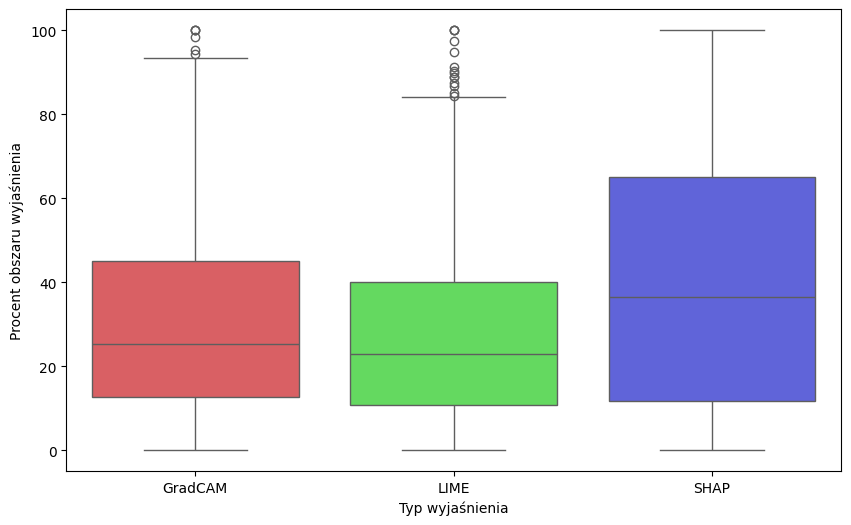
\includegraphics[width=.9\textwidth]{img/areaincorrect_vehicle}
		\caption{Vehicle}
	\end{subfigure}
	\begin{subfigure}[b]{0.3\textwidth}
		\centering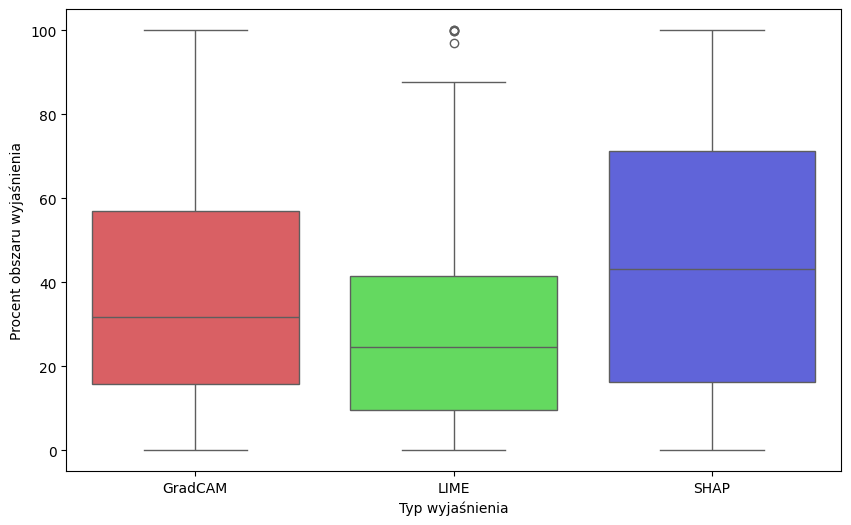
\includegraphics[width=.9\textwidth]{img/areaincorrect_reptile}
		\caption{Reptile}
	\end{subfigure}
	\begin{subfigure}[b]{0.3\textwidth}
		\centering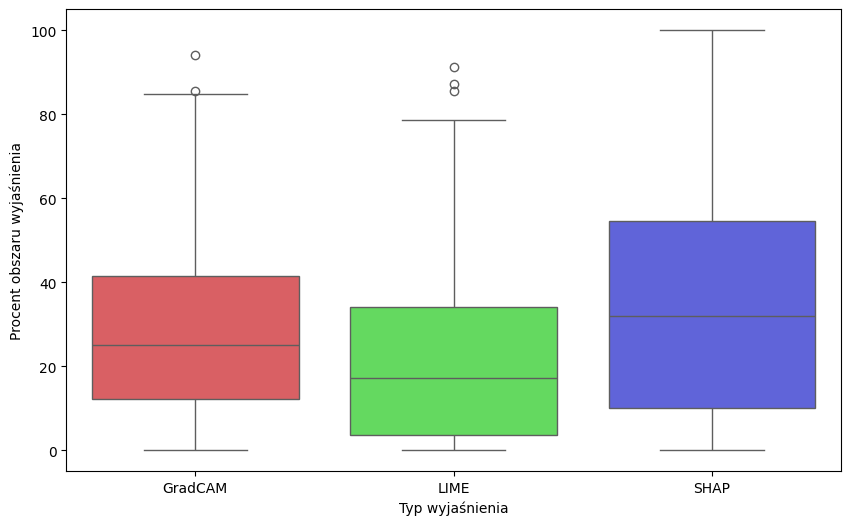
\includegraphics[width=.9\textwidth]{img/areaincorrect_carnivore}
		\caption{Carnivore}
	\end{subfigure}
	\begin{subfigure}[b]{0.3\textwidth}
		\centering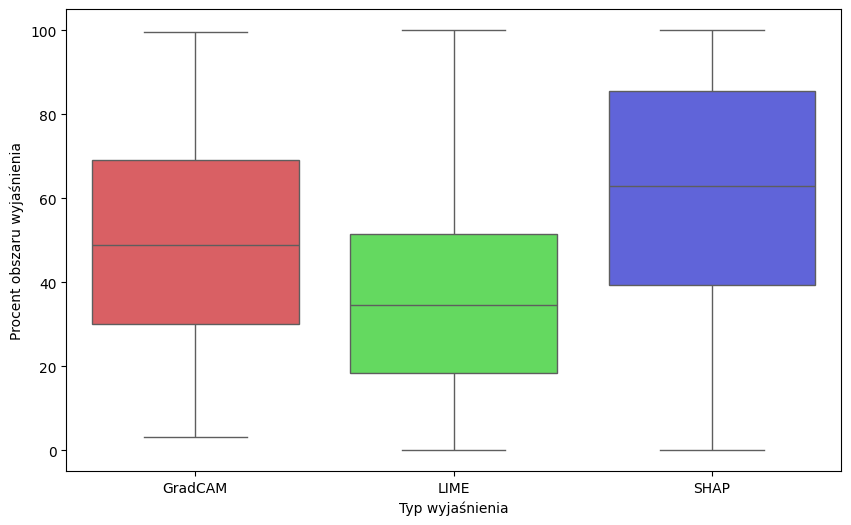
\includegraphics[width=.9\textwidth]{img/areaincorrect_insect}
		\caption{Insect}
	\end{subfigure}
	\begin{subfigure}[b]{0.3\textwidth}
		\centering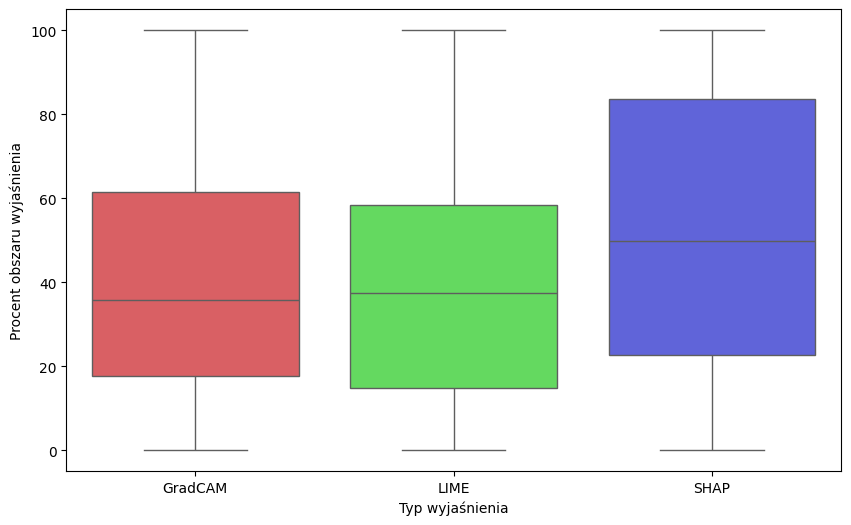
\includegraphics[width=.9\textwidth]{img/areaincorrect_music}
		\caption{Instrument}
	\end{subfigure}
	\begin{subfigure}[b]{0.3\textwidth}
		\centering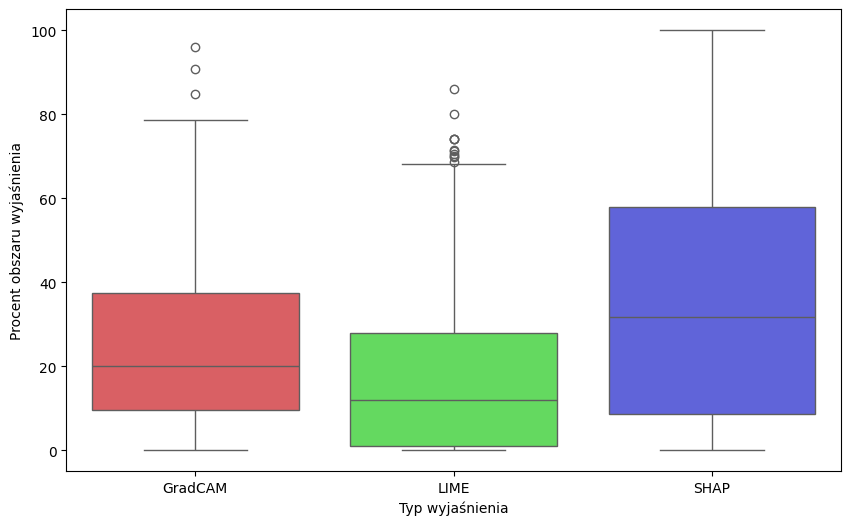
\includegraphics[width=.9\textwidth]{img/areaincorrect_primate}
		\caption{Primate}
	\end{subfigure}
	\begin{subfigure}[b]{0.3\textwidth}
		\centering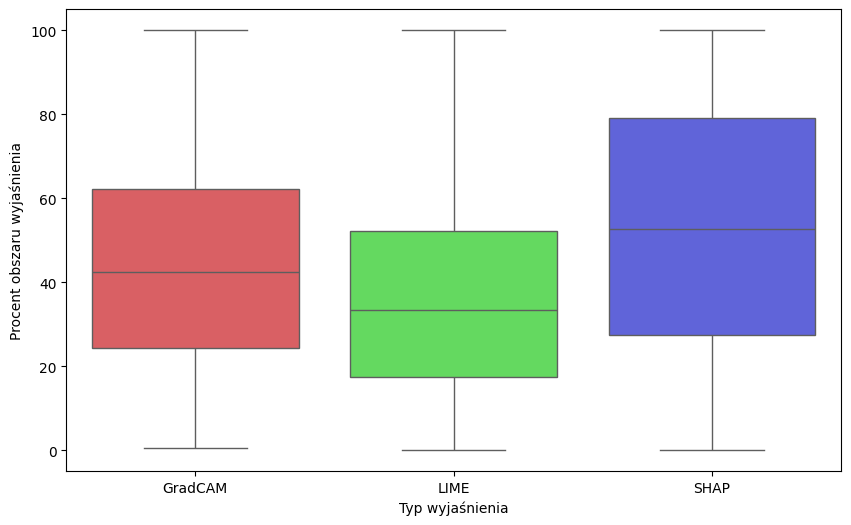
\includegraphics[width=.9\textwidth]{img/areaincorrect_fish}
		\caption{Fish}
	\end{subfigure}
	\caption{Procent obszaru wyjaśnienia poza obiektem}
	\label{rys:areaincorrect_category}
\end{figure}

\begin{table}[h]
	\centering
	\begin{tabular}{|c|c|c|c|}
		\hline
		\textbf{Kategoria}           & \textbf{GradCAM} & \textbf{LIME} & \textbf{SHAP} \\
		\hline
		\textbf{Pies}                & 22.727765\%      & 15.608602\%   & 32.742012\%   \\
		\hline
		\textbf{Ptak}                & 44.389150\%      & 34.211208\%   & 53.824976\%   \\
		\hline
		\textbf{Pojazd na kołach}    & 31.756452\%      & 28.022858\%   & 39.598063\%   \\
		\hline
		\textbf{Gad}                 & 37.630000\%      & 27.926620\%   & 45.545502\%   \\
		\hline
		\textbf{Mięsożerca}          & 28.788019\%      & 20.999559\%   & 34.912974\%   \\
		\hline
		\textbf{Insekt}              & 50.101927\%      & 36.614944\%   & 61.524663\%   \\
		\hline
		\textbf{Instrument muzyczny} & 41.103004\%      & 39.156369\%   & 52.134963\%   \\
		\hline
		\textbf{Naczelny}            & 25.07336\%       & 17.63363\%    & 36.43725\%    \\
		\hline
		\textbf{Ryba}                & 45.224726\%      & 36.728101\%   & 53.590312\%   \\
		\hline
	\end{tabular}
	\caption{Średni procent obszaru wyjaśnienia poza obiektem}
	\label{tab:areaincorrect_category}
\end{table}

Wyniki analizy  przedstawiono na wykresach (Rys. \ref{rys:areaincorrect_category}) oraz w Tabeli \ref{tab:areaincorrect_category}, która zawiera średnie procenty obszarów wyjaśnienia poza obiektami dla poszczególnych metod XAI i kategorii.

Metoda \textbf{GradCAM} często generuje wyjaśnienia, których obszar wykracza poza geanice obiektów na obrazie.
W niektórych kategoriach takich jak \textit{Insekt, Ryba i Ptak}, średni procent obszaru wyjaśnienia poza obiektem był bardzo wysoki.
Dla kategorii \textit{Pies} średni procent był najmniejszy.

Metoda \textbf{LIME} wygenerowała wyjaśnienia z najmniejszym procentem poza rzeczywistym obszarem obiektu, nizależnie od kategori.
Najlepsze wyniki dla LIME uzyskały kategorie \textit{Pies} oraz \textit{Naczelny}, natomiast najgorsze kategoria \textit{Instrument muzyczny}.

Metoda \textbf{SHAP} wygenerowała najgorsze wyjaśnienia.
Najgorszą kategorią były \textit{Insekt}, \textit{Ptak}, \textit{Instrument muzyczny} oraz \textit{Ryba}, gdzie średnio większość wyjaśnienia znajdowała się poza obiektem.

Porównując wyniki z wynikiami otrzymanymi dla całego zbioru, zauważono, że dla kategorii \textit{Pies}, \textit{Pojazdy na kołach}, \textit{Mięsożerca}, \textit{Naczelny} wszystkie metody osiągnęly lepsze wyniki.
Natomiast dla kategorii \textit{Gad} SHAP i LIME osiągneły lepsze wyniki
Dla pozostałych kategorii wszystkie metody osiągnęly gorsze wyniki.

\vspace{1cm}

Analiza zmiany pewności po pozostawieniu jedynie obszaru wyjaśnień z podziałem na kategorie pozwoliła na dokładniejsze badanie wpływu obszarów wyjaśnień na wynik modelu.

\begin{figure}[h]
	\centering
	\begin{subfigure}[b]{0.3\textwidth}
		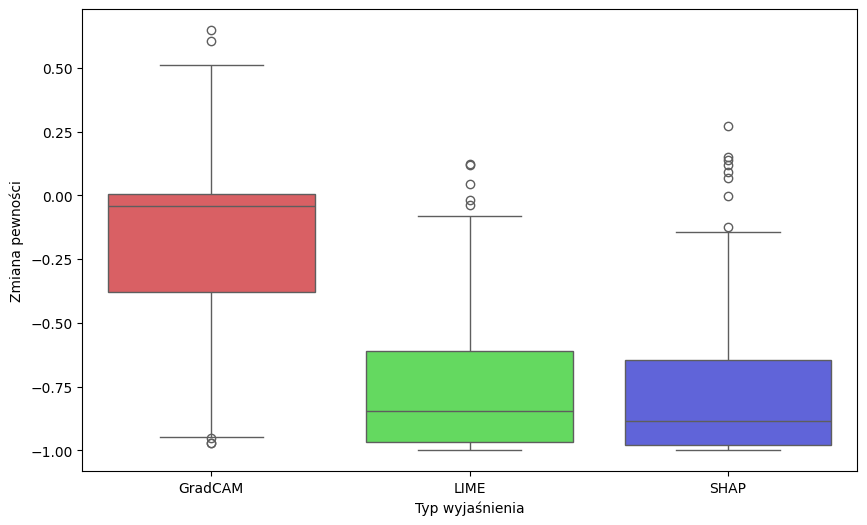
\includegraphics[width=.9\textwidth]{img/base_confidence_exp_dog}
		\caption{Dog}  \label{rys:base_confidence_exp_dog}
	\end{subfigure}
	\begin{subfigure}[b]{0.3\textwidth}
		\centering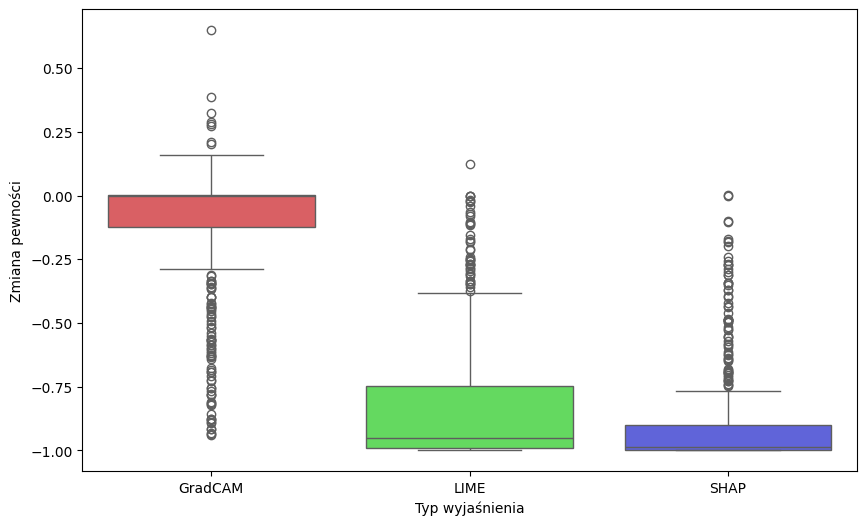
\includegraphics[width=.9\textwidth]{img/base_confidence_exp_bird}
		\caption{Bird}  \label{rys:base_confidence_exp_bird}
	\end{subfigure}
	\begin{subfigure}[b]{0.3\textwidth}
		\centering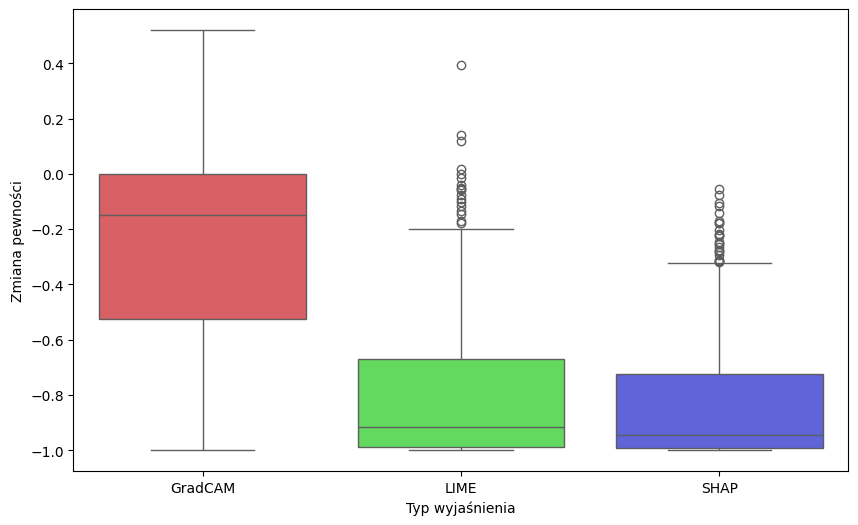
\includegraphics[width=.9\textwidth]{img/base_confidence_exp_vehicle}
		\caption{Vehicle}  \label{rys:base_confidence_exp_vehicle}
	\end{subfigure}
	\begin{subfigure}[b]{0.3\textwidth}
		\centering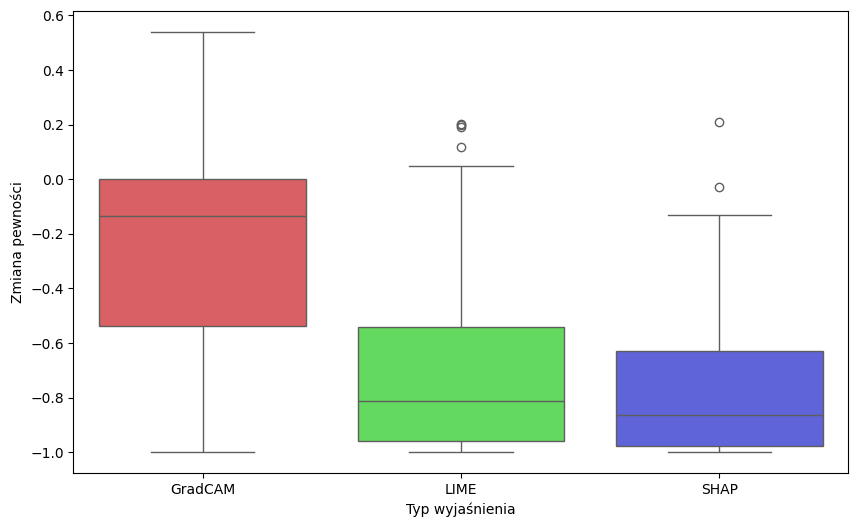
\includegraphics[width=.9\textwidth]{img/base_confidence_exp_reptile}
		\caption{Reptile}  \label{rys:base_confidence_exp_reptile}
	\end{subfigure}
	\begin{subfigure}[b]{0.3\textwidth}
		\centering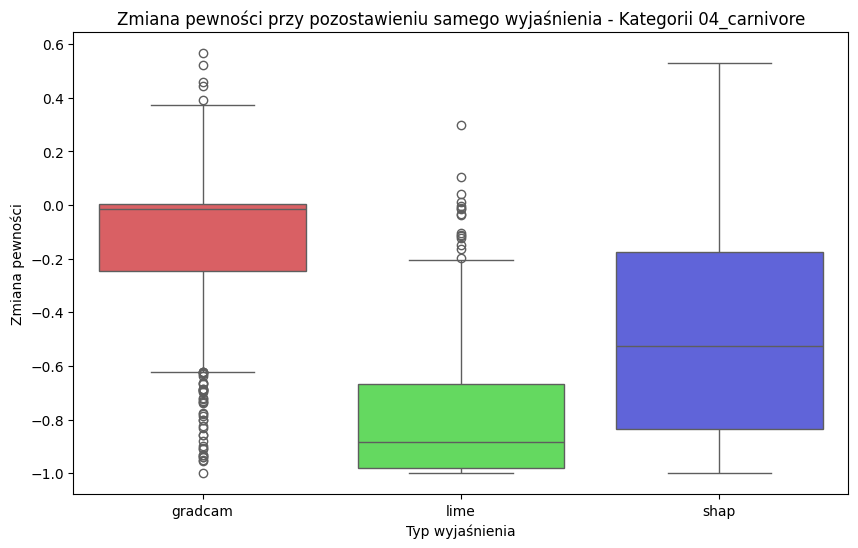
\includegraphics[width=.9\textwidth]{img/base_confidence_exp_carnivore}
		\caption{Carnivore}  \label{rys:base_confidence_exp_carnivore}
	\end{subfigure}
	\begin{subfigure}[b]{0.3\textwidth}
		\centering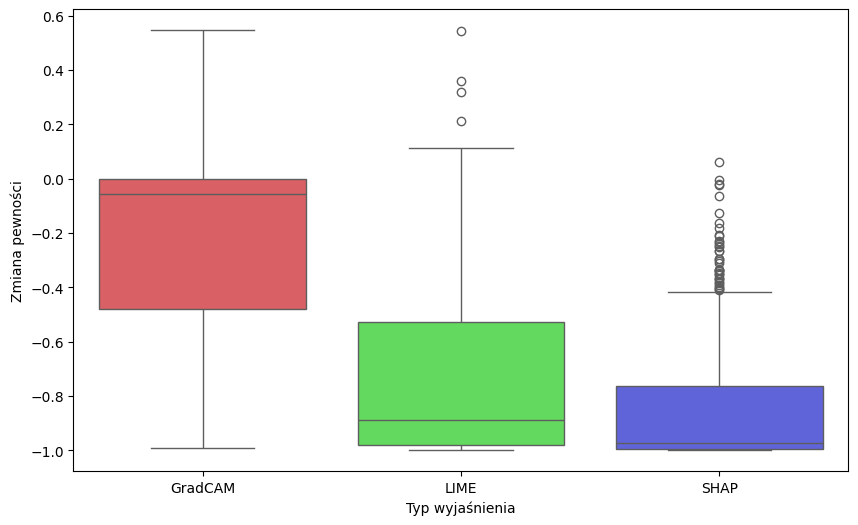
\includegraphics[width=.9\textwidth]{img/base_confidence_exp_insect}
		\caption{Insect}  \label{rys:base_confidence_exp_insect}
	\end{subfigure}
	\begin{subfigure}[b]{0.3\textwidth}
		\centering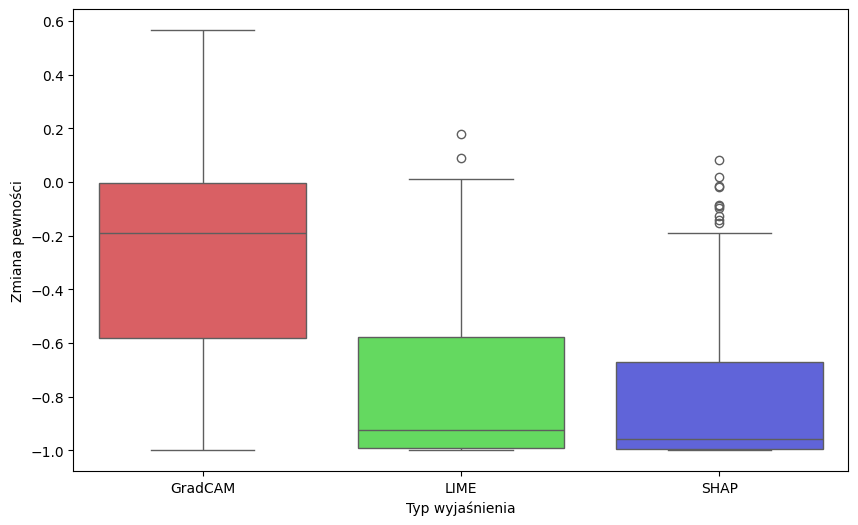
\includegraphics[width=.9\textwidth]{img/base_confidence_exp_music}
		\caption{Instrument}  \label{rys:base_confidence_exp_music}
	\end{subfigure}
	\begin{subfigure}[b]{0.3\textwidth}
		\centering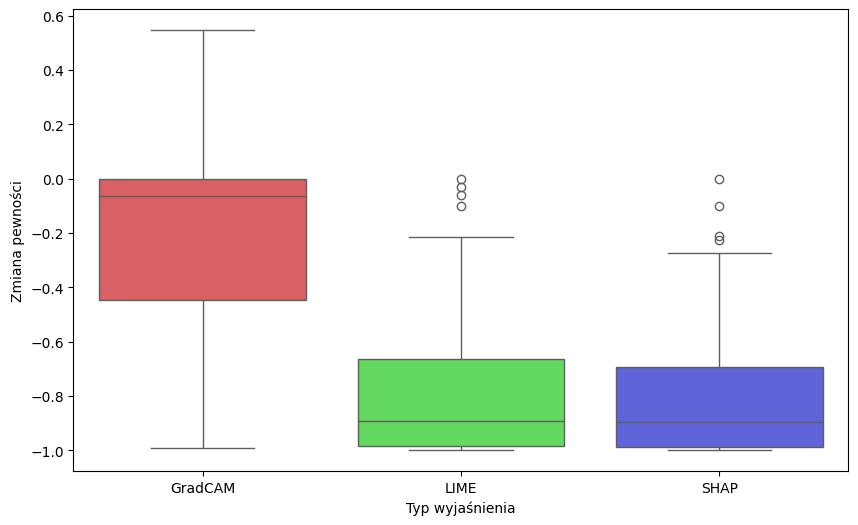
\includegraphics[width=.9\textwidth]{img/base_confidence_exp_primate}
		\caption{Primate}  \label{rys:base_confidence_exp_primate}
	\end{subfigure}
	\begin{subfigure}[b]{0.3\textwidth}
		\centering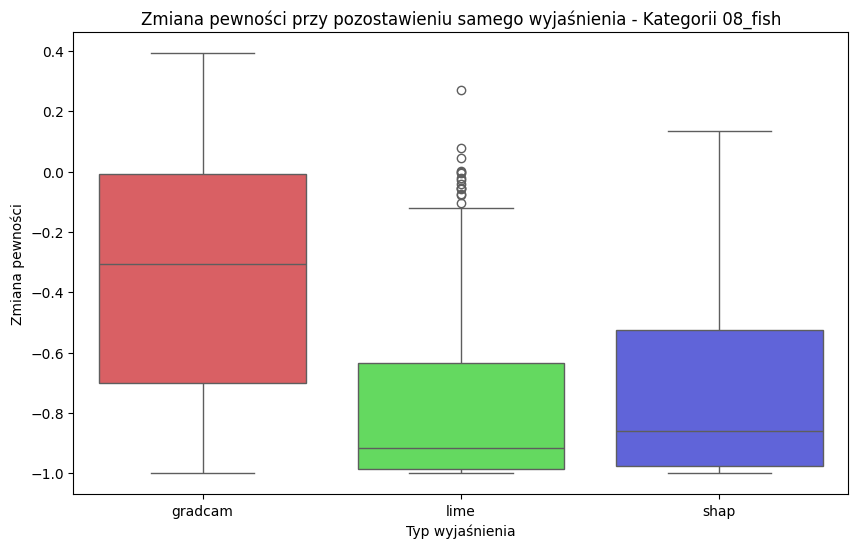
\includegraphics[width=.9\textwidth]{img/base_confidence_exp_fish}
		\caption{Fish}  \label{rys:base_confidence_exp_fish}
	\end{subfigure}
	\caption{Zmiana pewności po pozostawieniu jedynie obszatu wyjaśnienia dla różnych kategorii}
	\label{rys:base_confidence_exp_category}
\end{figure}

\begin{table}[h]
	\centering
	\begin{tabular}{|c|c|c|c|}
		\hline
		\textbf{Kategoria}           & \textbf{GradCAM} & \textbf{LIME} & \textbf{SHAP} \\
		\hline
		\textbf{Pies}                & -0.203837        & -0.770963     & -0.794431     \\
		\hline
		\textbf{Ptak}                & -0.126917        & -0.820506     & -0.891384     \\
		\hline
		\textbf{Pojazd na kołami}    & -0.283471        & -0.791623     & -0.822829     \\
		\hline
		\textbf{Gad}                 & -0.281027        & -0.732984     & -0.783735     \\
		\hline
		\textbf{Mięsożerca}          & -0.165199        & -0.798678     & -0.837208     \\
		\hline
		\textbf{Insekt}              & -0.244699        & -0.734359     & -0.844176     \\
		\hline
		\textbf{Instrument muzyczny} & -0.315661        & -0.768455     & -0.814664     \\
		\hline
		\textbf{Naczelny}            & -0.236171        & -0.800441     & -0.813812     \\
		\hline
		\textbf{Ryba}                & -0.374784        & -0.812877     & -0.839997     \\
		\hline
	\end{tabular}
	\caption{Średni spadek pewności modelu po pozostawieniu jedynie obszaru wyjaśnienia dla kategorii}
	\label{tab:category_confidence_exp}
\end{table}

\begin{table}[h]
	\centering
	\begin{tabular}{|c|c|c|c|}
		\hline
		\textbf{Kategoria}           & \textbf{GradCAM} & \textbf{LIME} & \textbf{SHAP} \\
		\hline
		\textbf{Pies}                & 32.8889\%        & 0.6667\%      & 1.3333\%      \\
		\hline
		\textbf{Ptak}                & 35.3333\%        & 0.2222\%      & 0.2222\%      \\
		\hline
		\textbf{Pojazd na kołami}    & 20.0000\%        & 0.8889\%      & 0.0000\%      \\
		\hline
		\textbf{Gad}                 & 25.5556\%        & 2.2222\%      & 0.2222\%      \\
		\hline
		\textbf{Mięsożerca}          & 31.5556\%        & 0.6667\%      & 0.0000\%      \\
		\hline
		\textbf{Insekt}              & 23.1111\%        & 2.4444\%      & 0.2222\%      \\
		\hline
		\textbf{Instrument muzyczny} & 14.8889\%        & 0.6667\%      & 0.4444\%      \\
		\hline
		\textbf{Naczelny}            & 27.3333\%        & 0.0000\%      & 0.0000\%      \\
		\hline
		\textbf{Ryba}                & 12.6667\%        & 0.0000\%      & 0.2222\%      \\
		\hline
	\end{tabular}
	\caption{Procent przypadków, w których pewność się zwiększyła dla kategorii}
	\label{tab:category_confidence_exp_percent}
\end{table}

Wyniki analizy zmiany pewności po pozostawieniu jedynie obszaru wyjaśnienia dla różnych kategorii obrazów przedstawiono na wykresach (Rys. \ref{rys:base_confidence_exp_category}) oraz w Tabelach \ref{tab:category_confidence_exp} i \ref{tab:category_confidence_exp_percent}, które zawierają średni spadek pewności modelu oraz procent przypadków, w których pewność modelu się zwiększyła po usunięciu obszarów uznanych przez metodę za nieistotne.

Metoda \textbf{GradCAM} wykazuje najniższy spadek pewności oraz największy procent przypadków, w których pewność się zwiększyła niezależnie od kategorii.
Jest to spowodowane większym obszarem wyjaśnień w porównaniu do pozostałych metod.
Najmniejszy spadek pewności oraz największy procent zwiększenia się pewności zanotowano dla kategorii \textit{Ptak}, natomiast największy spadek oraz najmniejszy procent dla kategorii \textit{Ryba}.

\textbf{LIME} charakteryzuje się wyraźnie większym spadkiem pewności po pozostawieniu jedynie obszaru wyjaśnień.
Dla kategorii \textit{Ptak} odnotowano największy spadek pewności, natomista dla kategorii \textit{Gad} najmniejszy spadek pewności.
Procent przypadków, w których pewność się zwiększyła jest zerowy dla kategorii \textit{Ryba} oraz \textit{Naczelny}.

\textbf{SHAP} wygenerował wyjaśnienia powodujące największy spadek pewności niezależnie od kategorii.
Najmnijeszy spadek pewności uzyskała kategoria \textit{Pies}, największy natomiast kategoria \textit{Ptak}.
Dla trzech kategorii (\textit{Pojazd na kołach, Mięsożerca, Naczelny}) procent przypdaków w których zwiększyła się pewność jest równy zero.
Tylko dla kategorii \textit{Pies} procent przypadków wynosił więcej niż jeden procent.

Średni spadek pewności w porównaniu do średniego spadku dla całego zbioru zmnijeszył się dla kategorii \textit{Pies} dla wszystkich metod oraz zwiększył się dla kategori \textit{Ryba} dla wszystkich metod.

Metoda GradCAM dostarcza wyjaśnienia które są często wystarczające do predykcji, natomiast zarówno SHAP jak i LIME dostarczają wyjaśnienia z zbyt małą ilością informacji do poprawnej klasyfikacji.

\vspace{1cm}

Analiza średniego spadku pewności po usunięciu obszaru wyjasnienia pomogła ocenić wartość obszarów podczas predykcji modelu.

\begin{figure}[h]
	\centering
	\begin{subfigure}[b]{0.3\textwidth}
		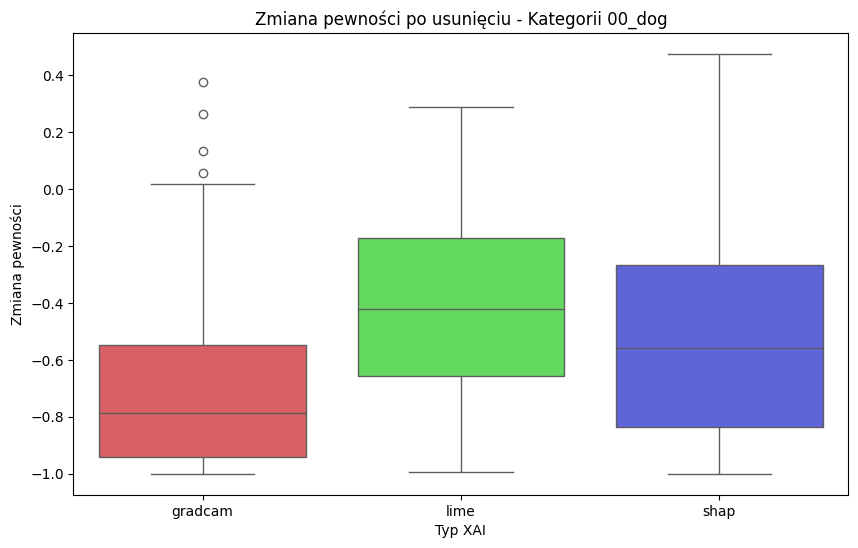
\includegraphics[width=.9\textwidth]{img/base_confidence_no_exp_dog}
		\caption{Dog}  \label{rys:base_confidence_no_exp_dog}
	\end{subfigure}
	\begin{subfigure}[b]{0.3\textwidth}
		\centering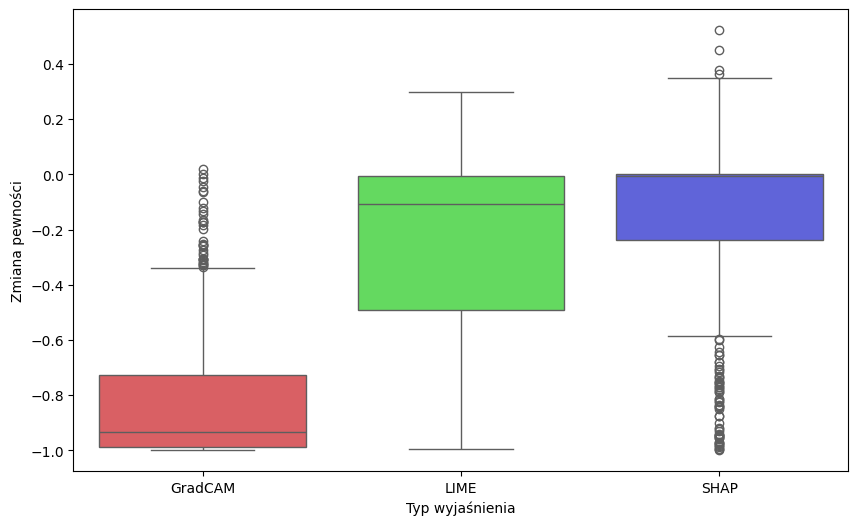
\includegraphics[width=.9\textwidth]{img/base_confidence_no_exp_bird}
		\caption{Bird}  \label{rys:base_confidence_no_exp_bird}
	\end{subfigure}
	\begin{subfigure}[b]{0.3\textwidth}
		\centering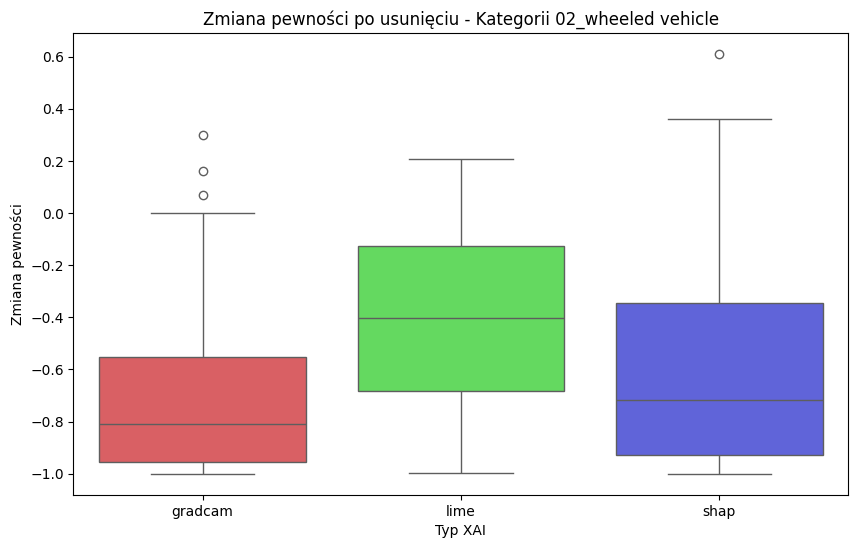
\includegraphics[width=.9\textwidth]{img/base_confidence_no_exp_vehicle}
		\caption{Vehicle}  \label{rys:base_confidence_no_exp_vehicle}
	\end{subfigure}
	\begin{subfigure}[b]{0.3\textwidth}
		\centering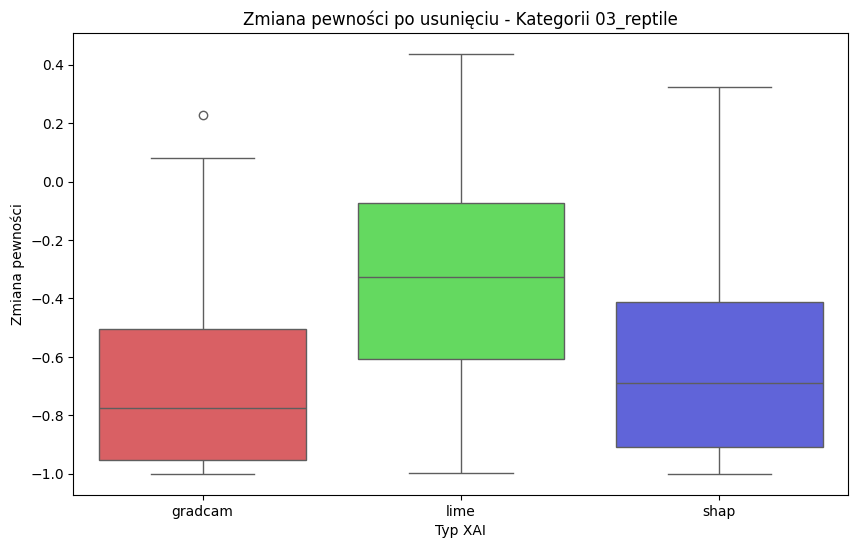
\includegraphics[width=.9\textwidth]{img/base_confidence_no_exp_reptile}
		\caption{Reptile}  \label{rys:base_confidence_no_exp_reptile}
	\end{subfigure}
	\begin{subfigure}[b]{0.3\textwidth}
		\centering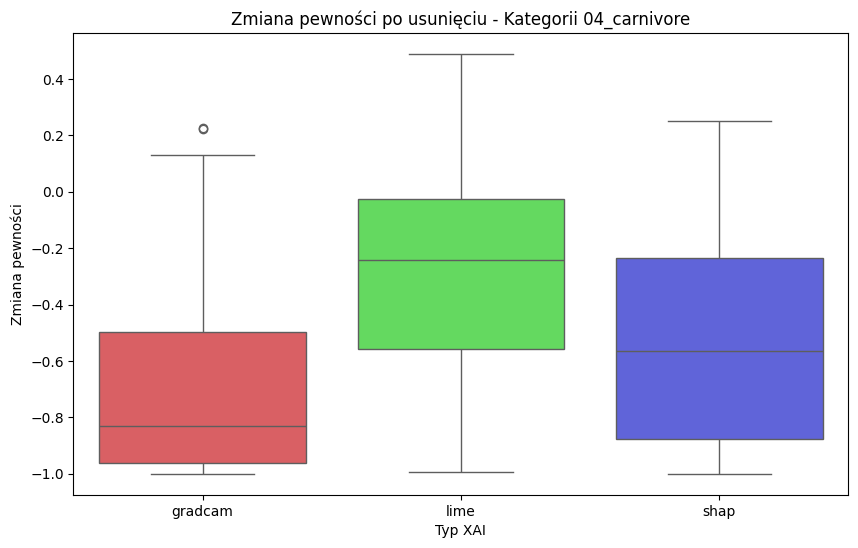
\includegraphics[width=.9\textwidth]{img/base_confidence_no_exp_carnivore}
		\caption{Carnivore}  \label{rys:base_confidence_no_exp_carnivore}
	\end{subfigure}
	\begin{subfigure}[b]{0.3\textwidth}
		\centering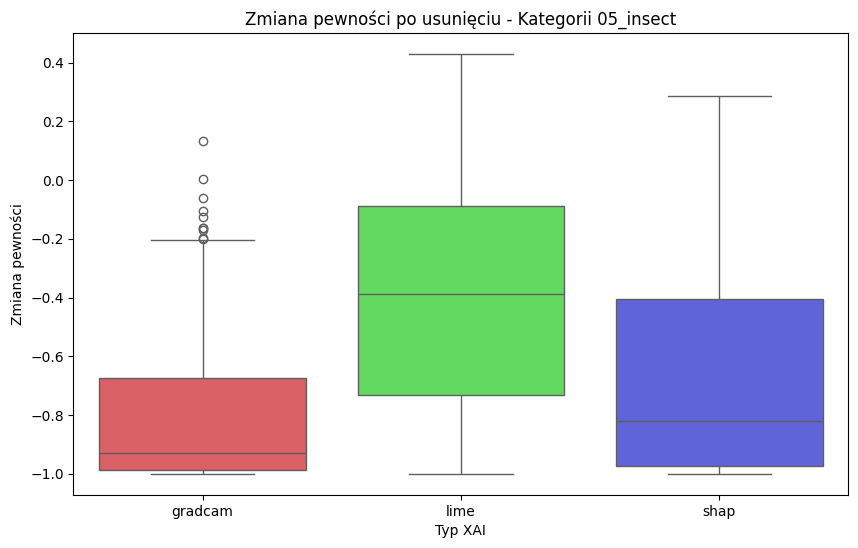
\includegraphics[width=.9\textwidth]{img/base_confidence_no_exp_insect}
		\caption{Insect}  \label{rys:base_confidence_no_exp_insect}
	\end{subfigure}
	\begin{subfigure}[b]{0.3\textwidth}
		\centering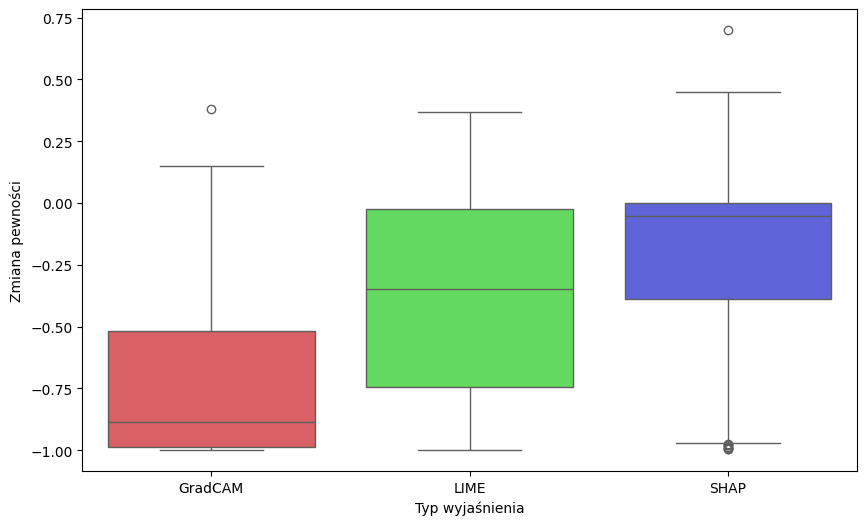
\includegraphics[width=.9\textwidth]{img/base_confidence_no_exp_music}
		\caption{Instrument}  \label{rys:base_confidence_no_exp_music}
	\end{subfigure}
	\begin{subfigure}[b]{0.3\textwidth}
		\centering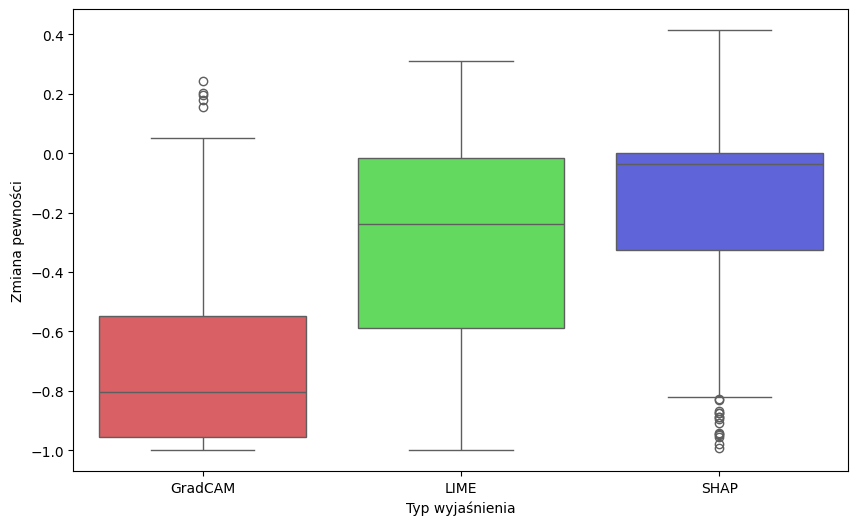
\includegraphics[width=.9\textwidth]{img/base_confidence_no_exp_primate}
		\caption{Primate}  \label{rys:base_confidence_no_exp_primate}
	\end{subfigure}
	\begin{subfigure}[b]{0.3\textwidth}
		\centering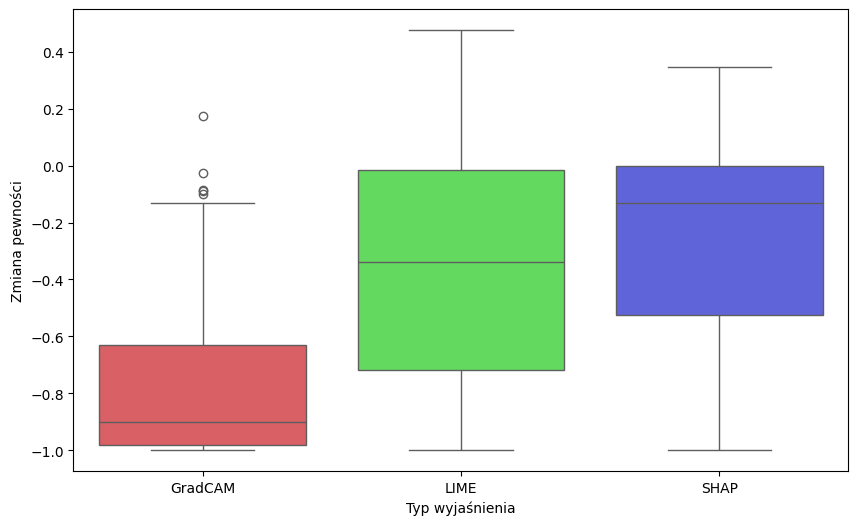
\includegraphics[width=.9\textwidth]{img/base_confidence_no_exp_fish}
		\caption{Fish}  \label{rys:base_confidence_no_exp_fish}
	\end{subfigure}
	\caption{Zmiana pewności po usunięciu obszaru wyjaśnienia dla różnych kategorii}
	\label{rys:category_confidence_no_exp}
\end{figure}

\begin{table}[h]
	\centering
	\begin{tabular}{|c|c|c|c|}
		\hline
		\textbf{Kategoria}           & \textbf{GradCAM} & \textbf{LIME} & \textbf{SHAP} \\
		\hline
		\textbf{Pies}                & -0.712184        & -0.336678     & -0.180713     \\
		\hline
		\textbf{Ptak}                & -0.815407        & -0.263471     & -0.181980     \\
		\hline
		\textbf{Pojazd na kołami}    & -0.731519        & -0.374297     & -0.166775     \\
		\hline
		\textbf{Gad}                 & -0.709709        & -0.365967     & -0.218283     \\
		\hline
		\textbf{Mięsożerca}          & -0.709833        & -0.268193     & -0.170374     \\
		\hline
		\textbf{Insekt}              & -0.802191        & -0.339857     & -0.219888     \\
		\hline
		\textbf{Instrument muzyczny} & -0.729714        & -0.405207     & -0.220832     \\
		\hline
		\textbf{Naczelny}            & -0.730957        & -0.332383     & -0.190197     \\
		\hline
		\textbf{Ryba}                & -0.786923        & -0.292582     & -0.289812     \\
		\hline
	\end{tabular}
	\caption{Średni spadek pewności modelu po usunięciu obszaru wyjaśnienia dla kategorii}
	\label{tab:category_confidence_no_exp}
\end{table}

Wyniki analizy zmiany pewności po usunięciu obszaru wyjaśnień dla różnych kategorii obrazów przedstawiono na wykresach (Rys. \ref{rys:category_confidence_no_exp}) oraz w Tabelach \ref{tab:category_confidence_no_exp}, które zawierają średni spadek pewności modelu.

Metoda \textbf{GradCAM} wykazuje największy spadek pewności modelu po usunięciu obszaru wyjaśnienia niezależnie od kategorii.
Największy spadek został zaobserowowany dla kategorii \textit{Ptak}, natomist najmniejsz dla kategorii \textit{Gad} oraz \textit{Mięsożerca}.

\textbf{LIME} wykazał największy spadek dla kategorii \textit{Instrument muzyczny}, natomiast najmniejszy dla kategorii \textit{Ptak} oraz \textit{Mięsożerca}.

\textbf{SHAP} wykazał najniższy spadek pewności modelu niezależnie od kategorii obrazu.
Największy spadek wykazał dla kategorii Rybam natomiast najmniejszy spadek dla kategorii Mięsożerca.

Porównując z analizą całego zbioru kategorie \textit{Pies}, \textit{Mięsożerca} i \textit{Naczelny} wykazały gorsze wyniki dla wszystkich metod XAI.

\vspace{1cm}

Analiza porównawcza wyjaśnień dla różnych kategorii obrazów pokazała, że metoda GradCAM często oferuje najlepszą lokalizację obszarów, pomimo dostarczania wyjaśnień często wykraczających poza obszar obiektu.
LIME i SHAP mają tendencję do generowania wyjaśnień mniejszych, nie wykrywających wystarczająco ogólnych cech.

\subsection*{Analiza w zależności od wielkość obiektu}

W tej sekcji dokonano analizy porownawczej metod GradCAM, LIME i SHAP pod względem generowanych wyjaśnień w zależności od wielkości obiektu na obrazie.
Analiza ta jest istotna, ponieważ wpływ wielkości obiektu na efektywność może się różnić w zależności od użytej metody XAI.
Podział na różne kategorie wielkości obiektów pozwala na ocenę, jak skutecznie każda metoda radzi sobie z generowaniem wyjaśnień dla różnych rozmiarów obeiektu.
Wyniki analizy dostarczyły informacji na temat elastyczności i dokładności poszczególnych metod.

\begin{figure}[h]
	\centering
	\begin{subfigure}[b]{0.3\textwidth}
		\centering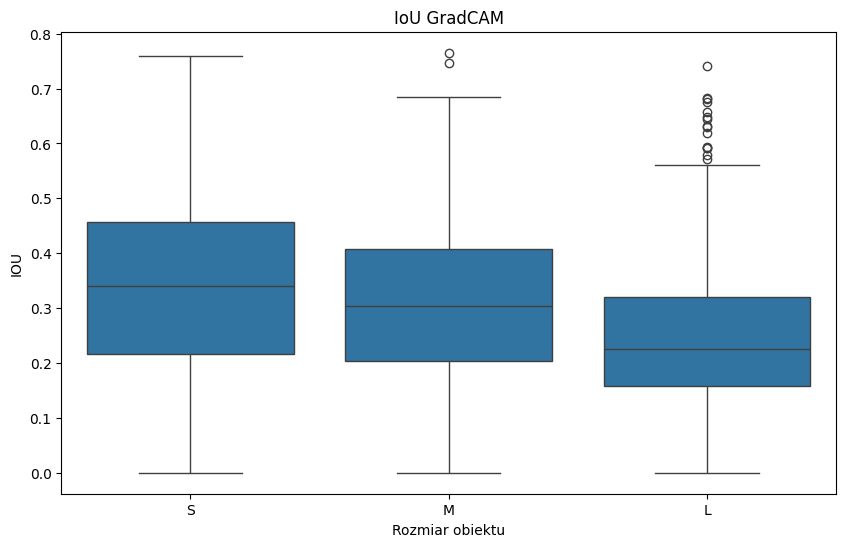
\includegraphics[width=.9\textwidth]{img/size_iou_gradcam}
		\caption{GradCAM}  \label{rys:size_iou_gradcam}
	\end{subfigure}
	\begin{subfigure}[b]{0.3\textwidth}
		\centering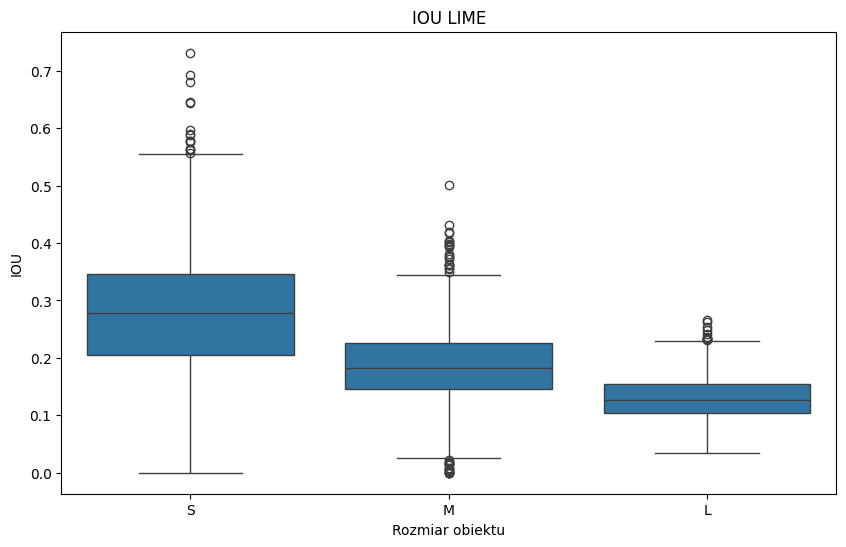
\includegraphics[width=.9\textwidth]{img/size_iou_lime}
		\caption{LIME}  \label{rys:size_iou_lime}
	\end{subfigure}
	\begin{subfigure}[b]{0.3\textwidth}
		\centering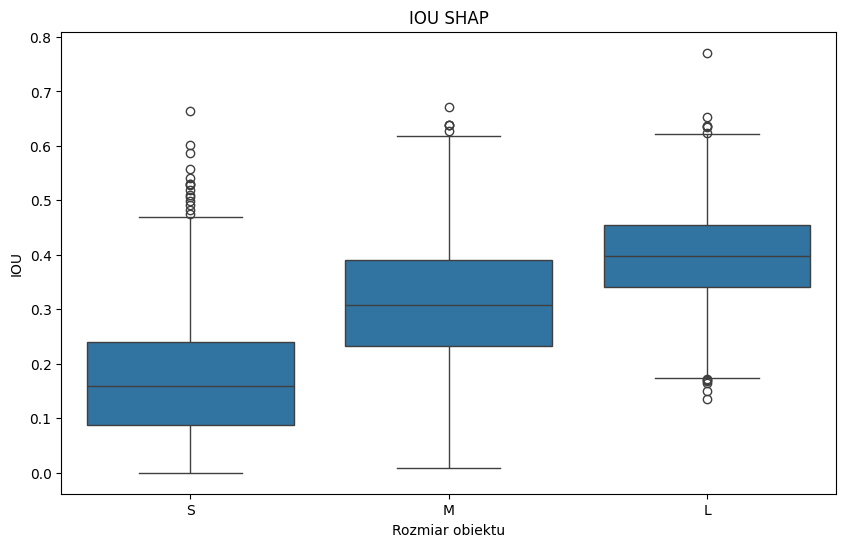
\includegraphics[width=.9\textwidth]{img/size_iou_shap}
		\caption{SHAP}  \label{rys:size_iou_shap}
	\end{subfigure}
	\caption{Wartości IoU w zależności od rozmiaru obiektu na obrazie}
	\label{rys:size_iou}
\end{figure}

\begin{table}[h]
	\centering
	\begin{tabular}{|c|c|c|c|}
		\hline
		\textbf{Rozmiar}     & \textbf{GradCAM} & \textbf{LIME} & \textbf{SHAP} \\
		\hline
		\textbf{Bardzo mały} & 0.050891         & 0.126901      & 0.035773      \\
		\hline
		\textbf{Mały}        & 0.354933         & 0.227675      & 0.117969      \\
		\hline
		\textbf{Średni}      & 0.477717         & 0.163982      & 0.122531      \\
		\hline
		\textbf{Duży}        & 0.496625         & 0.139437      & 0.118255      \\
		\hline
		\textbf{Bardzo duży} & 0.522507         & 0.131985      & 0.118691      \\
		\hline
	\end{tabular}
	\caption{Średnie wartości IoU w zależności od rozmiaru obiektu na obrazie}
	\label{tab:size_iou}
\end{table}

Wyniki analizy IoU dla różnych wielkości obiektów obrazów przedstawiono na wykresach (Rys. \ref{rys:size_iou}) oraz w Tabeli \ref{tab:size_iou}, która zawiera średnie wartości IoU.

\textbf{GradCAM} wykazał wyraźny wzrost wartości IoU wraz ze wzrostem wielkości obiektu.
Dla bardzo małych i małych obiektów zależność od wielkości ostatniej warstwy konwolucyjnej była najbardziej widoczna.

\textbf{LIME} uzyskał najlepsze wyniki ze wszystkich technik dla bardzo małych obiektów.
Najlepszy wynik uzyskał dla małych obiektów.
Następnie zmniejszała się ta wartość wraz ze wzrostem rozmiarów obiektu.

\textbf{SHAP} osiągnął nagorszy wynik dla obiektów bardzo małych, pozostałe rozmiary obiektów miały podobne wyniki.

GradCAM wykazuje najlepsze wyniki w zakresie pokrycia istotnych obszarów decyzyjnych na obrazach, zwłąszcza w przypadku większych obiektów.
LIME ma tendencję do generowania bardziej precyzyjnych wyjaśnień dla mniejszych obiektów, ale traci na efektywności dla większych.
SHAP ma najniższe wartości IOU, co może ograniczać jego zastosowanie.

\vspace{1cm}



\begin{figure}
	\centering
	\begin{subfigure}{0.3\textwidth}
		\centering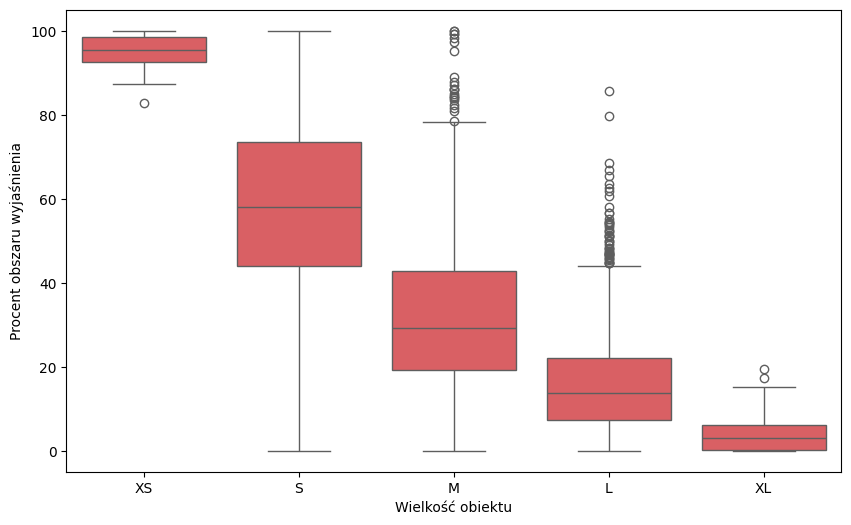
\includegraphics[width=.9\textwidth]{img/areaincorrect_size_gradcam}
		\caption{GradCAM}  \label{rys:areaincorrect_size_gradcam}
	\end{subfigure}
	\begin{subfigure}{0.3\textwidth}
		\centering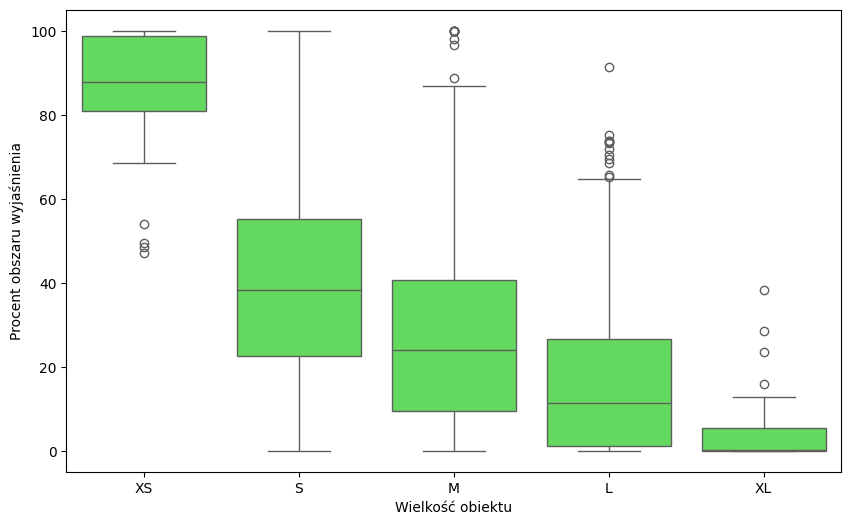
\includegraphics[width=.9\textwidth]{img/areaincorrect_size_lime}
		\caption{LIME}  \label{rys:areaincorrect_size_lime}
	\end{subfigure}
	\begin{subfigure}{0.3\textwidth}
		\centering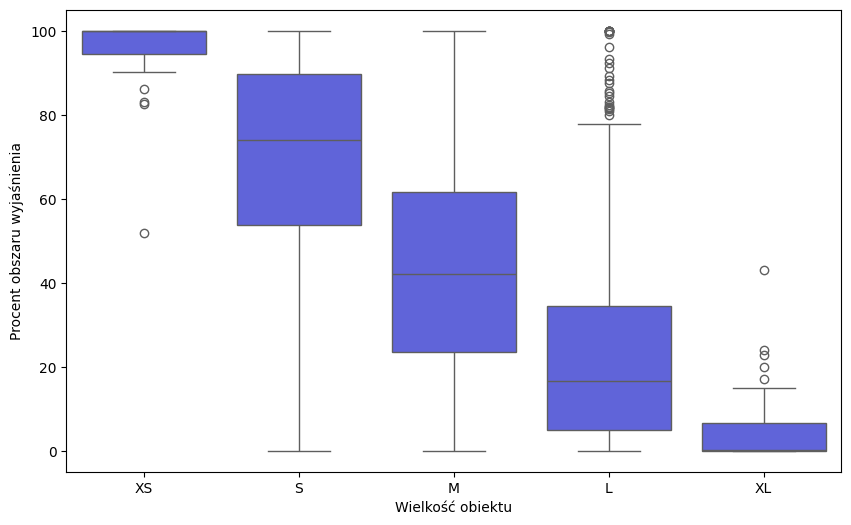
\includegraphics[width=.9\textwidth]{img/areaincorrect_size_shap}
		\caption{SHAP}  \label{rys:areaincorrect_size_shap}
	\end{subfigure}
	\label{rys:areaincorrect_size}
\end{figure}

\begin{table}[h]
	\centering
	\begin{tabular}{|c|c|c|c|}
		\hline
		\textbf{Rozmiar}     & \textbf{GradCAM} & \textbf{LIME} & \textbf{SHAP} \\
		\hline
		\textbf{Bardzo mały} & 94.901906        & 85.985901     & 95.942452     \\
		\hline
		\textbf{Mały}        & 58.767365        & 40.634976     & 69.416491     \\
		\hline
		\textbf{Średni}      & 32.141339        & 27.179856     & 43.712921     \\
		\hline
		\textbf{Duży}        & 16.371432        & 16.118421     & 22.106995     \\
		\hline
		\textbf{Bardzo duży} & 4.259065         & 4.566799      & 4.921229      \\
		\hline
	\end{tabular}
	\caption{Procent obszaru wyjaśnienia poza obiektem}
	\label{tab:size_area}
\end{table}

Wyniki analizy procentu obszaru poza obiektem dla różnych wielkości obiektów obrazów przedstawiono na wykresach (Rys. \ref{rys:areaincorrect_size}) oraz w Tabeli \ref{tab:size_area}, która zawiera średnie wartości precentu obaszarów poza obiektem.

Zgodnie z założeniami najmniejsze obiekty powodowały największy procent obszaru wyjaśnienia poza obiektem.
Najlepiej poradził sobie z tym LIME, który posiadał najlepsze wyniki dla wszystkich wielkości poza Bardzo dużymi obiektami, gdzie GradCAM miał marginalnie lepsze wyniki, przy czym należy pamiętać że w grupie bardzo dużych obiektów jest relatywnie mała ilość obrazów.

\vspace{1cm}

\textbf{Zmiana pewności przy pozostawieniu samego wyjaśnienia}
\begin{figure}[h]
	\centering
	\begin{subfigure}[b]{0.3\textwidth}
		\centering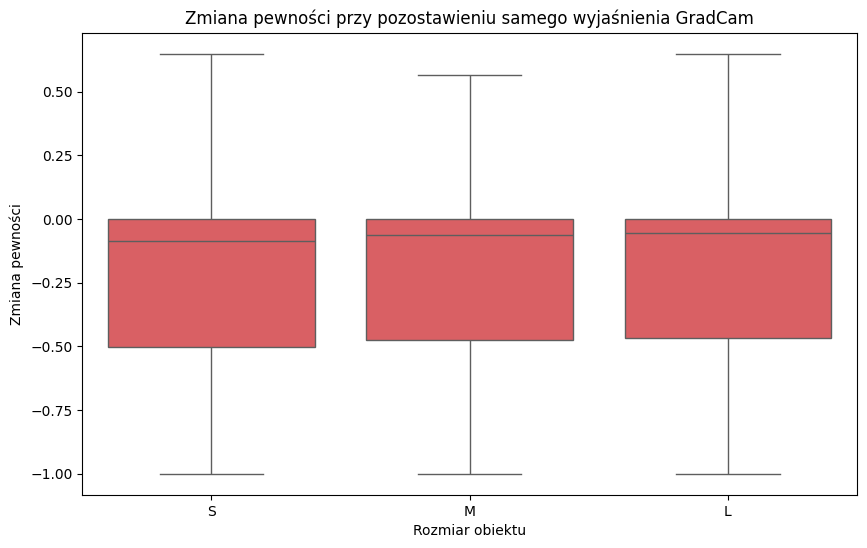
\includegraphics[width=.9\textwidth]{img/size_confidence_exp_gradcam}
		\caption{GradCAM}  \label{rys:size_confidence_mask_gradcam}
	\end{subfigure}
	\begin{subfigure}[b]{0.3\textwidth}
		\centering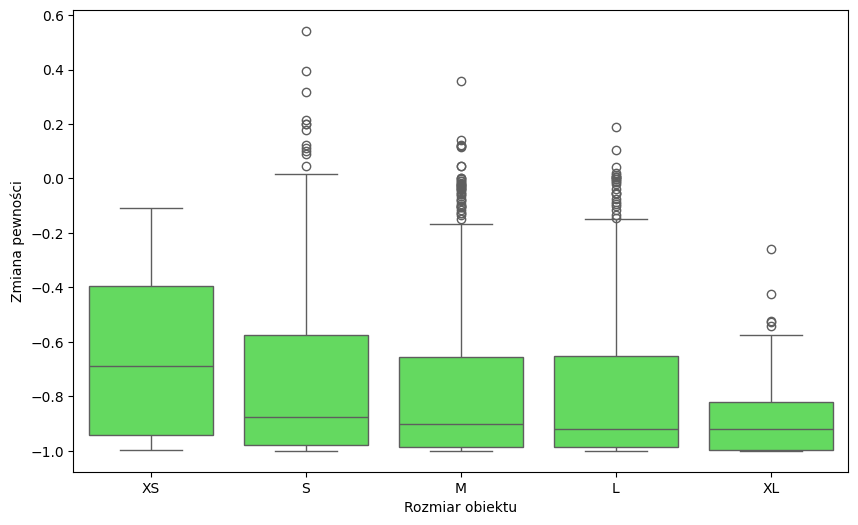
\includegraphics[width=.9\textwidth]{img/size_confidence_exp_lime}
		\caption{LIME}  \label{rys:size_confidence_mask_lime}
	\end{subfigure}
	\begin{subfigure}[b]{0.3\textwidth}
		\centering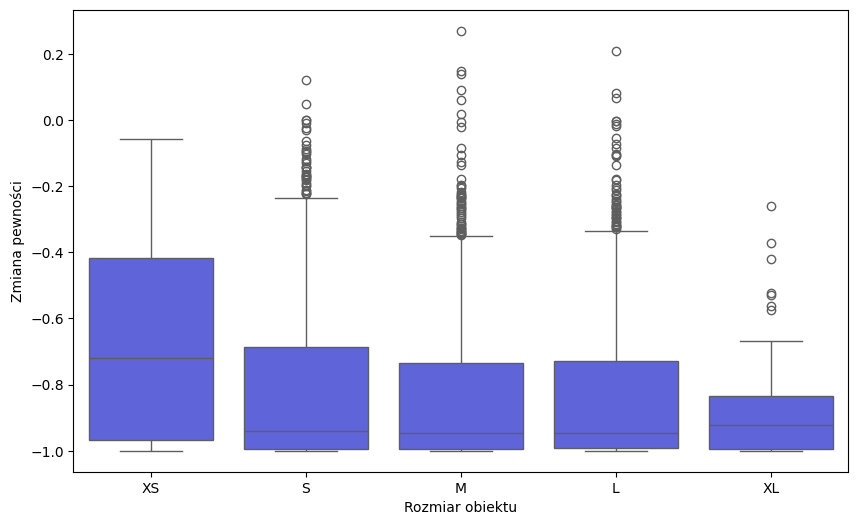
\includegraphics[width=.9\textwidth]{img/size_confidence_exp_shap}
		\caption{SHAP}  \label{rys:size_confidence_mask_shap}
	\end{subfigure}
	\caption{Zmiana pewności przy usunięciu obszarów wyjaśnienia}
	\label{rys:size_confidence_exp}
\end{figure}

\begin{table}[h]
	\centering
	\begin{tabular}{|c|c|c|c|}
		\hline
		\textbf{Rozmiar}     & \textbf{GradCAM} & \textbf{LIME} & \textbf{SHAP} \\
		\hline
		\textbf{Bardzo mały} & -0.369749        & -0.637539     & -0.657654     \\
		\hline
		\textbf{Mały}        & -0.259113        & -0.750735     & -0.812674     \\
		\hline
		\textbf{Średni}      & -0.242182        & -0.791863     & -0.838422     \\
		\hline
		\textbf{Duży}        & -0.239186        & -0.803234     & -0.833250     \\
		\hline
		\textbf{Bardzo duży} & -0.232523        & -0.861181     & -0.860782     \\
		\hline
	\end{tabular}
	\caption{Zmiana pewności przy samym obszarze wyjaśnienia w zależności od rozmiaru obiektu na obrazie}
	\label{tab:size_confidence_exp}
\end{table}

\begin{table}[h]
	\centering
	\begin{tabular}{|c|c|c|c|}
		\hline
		\textbf{Rozmiar}     & \textbf{GradCAM} & \textbf{LIME} & \textbf{SHAP} \\
		\hline
		\textbf{Bardzo mały} & 02.3256\%        & 00.0000\%     & 00.0000\%     \\
		\hline
		\textbf{Mały}        & 23.3896\%        & 01.3804\%     & 00.2301\%     \\
		\hline
		\textbf{Średni}      & 26.3048\%        & 00.6263\%     & 00.4175\%     \\
		\hline
		\textbf{Duży}        & 25.5947\%        & 00.6563\%     & 00.2461\%     \\
		\hline
		\textbf{Bardzo duży} & 19.1489\%        & 00.0000\%     & 00.0000\%     \\
		\hline
	\end{tabular}
	\caption{Procent przypadków, w których pewność się zwiększyła sam obszar wyjaśnienia dla rozmirów}
	\label{tab:size_confidence_exp_percent}
\end{table}

Wyniki analizy zmiany pewności po pozostawieniu jedynie obszarów wyjaśnienia dla różnych wielkości obiektów obrazów przedstawiono na wykresach (Rys. \ref{rys:size_confidence_exp}) oraz w Tabelach \ref{tab:size_confidence_exp} oraz \ref{tab:size_confidence_exp_percent}.

Średni spadek pewności modelu jest najmniejszy zawsze dla \textbf{GradCAM}.
Najmniejszy jest dla obszarów bardzo dużych po czym się zwiększa.
Procent przypdaków, w których pewność się zwiększyła jest zawsze największa dla GradCAM, przy czym dla bardzo małych jest ona zdecydowanie najmniejsza.

W przeciwieństwie do GradCAM, dla \textbf{LIME} pewność zwiększa się wraz ze wzrostem wielkości obiektu.
Co oznacza, że im mniejszy obiekt tym lepsze wyniki.
Procent przypadków, w których pewność się zwiększyła jest natomiast zawsze niski, w porównaniu do GradCAM jednak jest ona najwyższa dla obiektów małych.

W przypadku \textbf{SHAP} najmniejsze zmiana jest dla obiektów bardzo małych, natomiast największa dla bardzo dużych.
Procent przypadków, w których pewność się zwiększyła jest zawsze niska, dla bardzo małych oraz bardzo dużych jest ona zerowa.

GradCAM okazuje się najskuteczniejszy w generowanu istotnych wyjaśnień, które mają prawdziwy wpływ na pewność modelu, zwłaszcza w przypadku średnich, dużych i bardzo dużych obiektów.

\vspace{1cm}

\textbf{Zmiana pewności po usunięciu obszarów wyjaśnień}
\begin{figure}[h]
	\centering
	\begin{subfigure}[b]{0.3\textwidth}
		\centering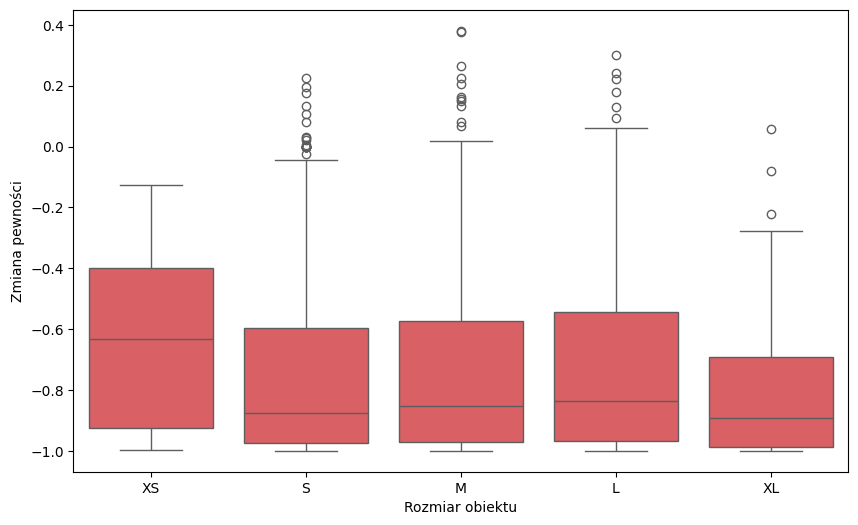
\includegraphics[width=.9\textwidth]{img/size_confidence_no_exp_gradcam}
		\caption{GradCAM}  \label{rys:size_confidence_no_exp_gradcam}
	\end{subfigure}
	\begin{subfigure}[b]{0.3\textwidth}
		\centering\includegraphics[width=.9\textwidth]{img/size_confidence_no_exp_lime}
		\caption{LIME}  \label{rys:size_confidence_no_exp_lime}
	\end{subfigure}
	\begin{subfigure}[b]{0.3\textwidth}
		\centering\includegraphics[width=.9\textwidth]{img/size_confidence_no_exp_shap}
		\caption{SHAP}  \label{rys:size_confidence_no_exp_shap}
	\end{subfigure}
	\caption{Zmiana pewności po usunięciu obszatu wyjaśnienia - rozmiar obiektu}
\end{figure}

\begin{table}[h]
	\centering
	\begin{tabular}{|c|c|c|c|}
		\hline
		\textbf{Rozmiar}     & \textbf{GradCAM} & \textbf{LIME} & \textbf{SHAP} \\
		\hline
		\textbf{Bardzo mały} & -0.617362        & -0.484938     & -0.298606     \\
		\hline
		\textbf{Mały}        & -0.763479        & -0.398575     & -0.253015     \\
		\hline
		\textbf{Średni}      & -0.749968        & -0.326675     & -0.177250     \\
		\hline
		\textbf{Duży}        & -0.730637        & -0.296358     & -0.180975     \\
		\hline
		\textbf{Bardzo duży} & -0.794106        & -0.299977     & -0.199899     \\
		\hline
	\end{tabular}
	\caption{Średni spadek po usunięciu obszaru wyjaśnienia dla rozmiarów}
	\label{tab:size_confidence_no_exp}
\end{table}

\textbf{GradCAM} wykazuje największy spadek pewności po usunięciu obszaru wyjaśnienia we wszystkich kategoriach wielkości obszaru.
Największy spadek obserwowany jest dla bardzo dużych obiektów, natomiast najmniejszy dla bardzo małych obiektów.

\textbf{LIME} generuje mniejsze spadki pewności w porównaniu do GradCAM szczególnie zauważalne przy średnich, dużych i bardzo dużych obiektach.
Najlepsze wyniki uzyskał dla bardzo małych obiektów.

\textbf{SHAP} wykazuje najmniejszy spadek pewności po usunięciu obszarów wyjaśnienia.

\textbf{GradCAM} generuje najbardziej istotne wyjaśnienia, które mają największy wpływ na pewność modelu, co jest szczególnie widoczne w przypadku bardzo dużych obiektów.
LIME, mimo że mniej skuteczny od GradCAM, wykazuje dobra przydatność dla bardzo małych obiektów.
SHAP wykazuje najgorsze wyniki niezależnie od wielkości obiektu.

\vspace{1cm}
Podsumowując GradCAM jest najbardziej efektywną metodą zwłaszcza dla większych obiektów.
Wyjaśnienia generowane przez GradCAM mają największy wpływ na decyzję modelu.
LIME generuje mniej efektywne wyjaśnienia, które są szczególnie użyteczne dla bardzo małych obiektów.
SHAP ma najniższą skuteczność w generowaniu wyjaśnień, wyjaśnienia są najmniej istotne dla decyzji modelu, co jest szczególnie widoczne dla bardzo małych i bardzo dużych obiektów.
